\documentclass[11pt,a4paper]{article}
\usepackage[margin=2.5cm]{geometry}
\linespread{1.15}
\setlength{\parskip}{0.5em}
\setlength{\parindent}{0pt}
\usepackage{amsmath,amssymb,amsthm,physics,graphicx,booktabs,hyperref}
\usepackage[capitalize]{cleveref}
\usepackage{enumitem,longtable}
\usepackage[section]{placeins}
\makeatletter\setlength{\@fptop}{0pt}\setlength{\@fpsep}{2.5em}\setlength{\@fpbot}{0pt plus 1fil}\makeatother
\setlist{itemsep=0.3em,topsep=0.3em}
\setlength{\emergencystretch}{2em}
\newtheorem{proposition}{Proposition}
\title{When Does Entanglement Give a Real Advantage?\\[2pt]
\large The CHSH Game, the Quantum Prisoner's Dilemma and Quantum Chess under Local Noise}
\author{Nihal Krishna Shrivastava \hspace{2.5em} Kishore Nagarajan}
\date{}

\begin{document}
\maketitle

\begin{abstract}
We compare two settings in which players share an entangled pair: the Clauser--Horne--Shimony--Holt (CHSH) nonlocal game, a cooperative game against a referee, and the Eisert--Wilkens--Lewenstein (EWL) quantum Prisoner's Dilemma, a non-cooperative game with an arbiter. For CHSH we prove the classical bound $3/4$ and the quantum value $\cos^2(\pi/8)\approx 0.854$ via Tsirelson's bound. For EWL we derive the payoffs, verify that $(D,D)$ is a Nash equilibrium (NE) for $\gamma\le\arcsin(1/\sqrt5)$ and $(Q,Q)$ for $\gamma\ge\arcsin\sqrt{2/5}$ within the two-parameter strategy set, and reproduce the mixed equilibria in the full $SU(2)$ set: a mixed NE with payoff $5/2$ (we prove that no deviation by either player pays more than $5/2$), and the weak focal equilibrium with payoff $9/4$. We then apply the three single-qubit channels of the course (depolarizing, dephasing, amplitude damping) to both games. With measurement settings optimised for the noisy state (Horodecki criterion), the CHSH violation is lost at $p^*=0.119$ for depolarizing noise and $p^*=1-1/\sqrt2=0.293$ for amplitude damping, and under dephasing it survives for every $p<1$, although its margin shrinks like $(1-p)^4$ for $p$ near 1. The EWL $(Q,Q)$ equilibrium survives for all tested noise strengths ($p\le0.6$), but needs more entanglement under depolarizing and dephasing noise and pays less; under dephasing at $\gamma=\pi/2$ we prove that it is lost exactly at $p=1-1/\sqrt7\approx0.622$. Its payoff stays above that of the classical equilibrium $(D,D)$ of the same noisy device for depolarizing noise and amplitude damping, but under dephasing $(D,D)$ itself stops being an equilibrium of the classical game above $p=1-1/\sqrt3\approx0.423$, and for $0.423<p\le0.622$ the new asymmetric classical equilibria give a higher average payoff than $(Q,Q)$. As a third, contrasting case we analyse the split and merge moves of quantum chess under the same three channels. We prove that the merge returns a coherently split piece with probability $\bra\psi\rho\ket\psi$, which beats a classical random move by $(1-p)^2/2$ under dephasing, $(1-p)/2$ under amplitude damping and $(1-\frac43p)^2/2$ under depolarizing noise. Under depolarizing noise this margin vanishes only at $p=3/4$, while the entanglement of the two squares is lost at $p=0.317$ and the CHSH violation at $p=0.119$. We argue that these ``advantages'' are of different kinds and discuss the van Enk--Pike and Landsburg critiques. The noiseless games are cross-checked in Qiskit; all noisy results come from numpy and SymPy code available in our public repository.
\end{abstract}

\section{Introduction}
Quantum game theory asks what changes when the moves of a game are quantum operations \cite{meyer,ewl,flitney-review}. Two lines of work exist. Nonlocal games such as CHSH (the inequality \cite{chsh} in its game form \cite{cleve}) are cooperative: two players who cannot communicate try to satisfy a referee, and shared entanglement raises their winning probability above anything classical. Quantum versions of classical games such as the Eisert--Wilkens--Lewenstein (EWL) Prisoner's Dilemma \cite{ewl} are non-cooperative: entanglement is introduced by an arbiter, and the question is which equilibria appear.

The second line has been criticised. Benjamin and Hayden showed that the $(Q,Q)$ equilibrium of EWL disappears when players may use any $SU(2)$ operation \cite{bh}. Van Enk and Pike \cite{vanenk} and Landsburg \cite{landsburg} argued that the quantum game is a different classical game with a larger payoff table. Our guiding question is therefore: \emph{in which of the two settings is the advantage of quantum origin, and how robust is each to the noise channels studied in this course?} As a third, contrasting case we include quantum chess \cite{cantwell}, where pieces can be split over two squares and merged back; there the quantum feature at work is coherence between the two branches of one piece, with no equilibrium or Bell test involved.

\paragraph{Contributions.} (i) Derivations of the CHSH bounds and the EWL equilibrium structure, self-contained except for three cited standard results (Naimark dilation, the Ky Fan inequality and the Horodecki formula); (ii) numerical checks of the analytic results that can be computed (payoffs, thresholds, bounds); (iii) a side-by-side study of both games under the same local channels (Topic 9 of the course notes), including optimised CHSH settings, whose thresholds differ from fixed-setting ones for amplitude damping and dephasing; (iv) a proof that the $9/4$ focal equilibrium of Eisert and Wilkens \cite{ew2000} is a weak equilibrium in which every strategy is a best response, which we have not reconciled with the classification of Bolonek-Laso\'n and Kosi\'nski \cite{bolonek}; (v) exact results under dephasing: the $(Q,Q)$ threshold $p=1-1/\sqrt7$, the point $p=1-1/\sqrt3$ above which $(D,D)$ stops being a classical equilibrium, and the quantum chess recovery probabilities under all three channels, and how they compare with the entanglement and CHSH thresholds of the same depolarized states. Prior studies of noisy EWL games exist \cite{johnson,chen,flitney-decoh}; to our knowledge, the common-channel comparison with CHSH is new.
\section{Notation}

{\small
\begin{longtable}{lp{0.45\linewidth}}
\toprule
$X,Y,Z$ & Pauli matrices; $\mathbb{I}$ identity\\
$\ket{\Phi^+}=(\ket{00}+\ket{11})/\sqrt2$ & Bell state used in CHSH\\
$\sigma_1,\sigma_2,\sigma_3$ & $X,Y,Z$; $\sigma_0=\mathbb I$\\
$A_x,B_y$ & $\pm1$ observables of Alice and Bob\\
$E_{xy}$ & correlator $\langle A_x\otimes B_y\rangle$\\
$S$ & CHSH value $E_{00}+E_{01}+E_{10}-E_{11}$, \cref{eq:S}\\
$S_{\max}$ & $S$ maximised over all settings\\
$T$ & correlation matrix $T_{ij}=\tr[\rho\,\sigma_i\otimes\sigma_j]$\\
$U(\theta,\phi)$ & EWL two-parameter strategy, \cref{eq:U}\\
$C=U(0,0),\ D=U(\pi,0),\ Q=U(0,\pi/2)=iZ$ & cooperate, defect, quantum move\\
$R$ & uniform mixture of $\{\mathbb{I},iX,iY,iZ\}$, \cref{prop:focal}\\
$J(\gamma)=\exp(i\gamma D\otimes D/2)$ & EWL entangling gate, $\gamma\in[0,\pi/2]$\\
$\$_A,\$_B$ & expected payoffs\\
$\mathcal E_p$ & single-qubit noise channel of strength $p$\\
$p^*$ & smallest $p$ with $S\le2$ (fixed settings) or $S_{\max}\le2$ (optimised settings)\\
$k=(1-p)^2$ & coherence factor of dephasing on two qubits\\
$\pi_{XY}$ & Alice's payoff at $(X,Y)$, $X,Y\in\{C,D\}$, $\gamma=\pi/2$ (\cref{sec:noise})\\
$W,V$ & quantum chess jump (iSWAP) and split gate ($\sqrt{\text{iSWAP}}$)\\
$\ket\psi,\ket{\psi_\perp}$ & split state of a chess piece and its orthogonal partner\\
$\rho_c$ & classical random move (50/50 mixture)\\
$P_q,P_c$ & recovery probability of the coherent split and of $\rho_c$\\
$\eta=1-\frac43p$, $v=\eta^2$ & depolarizing Bloch factor; its two-qubit square\\
$\ket{\Psi^+}$, $\mathcal N$ & $(\ket{01}+\ket{10})/\sqrt2$; negativity\\
$\mathcal M$ & quantum chess merge $V_{sa}W_{sb}$\\
\bottomrule
\end{longtable}}

\section{The CHSH game}

\subsection{Rules and the classical bound}
A referee sends uniformly random bits $x$ to Alice and $y$ to Bob. They answer $a,b\in\{0,1\}$ without communicating and win iff $a\oplus b=x\wedge y$.

\begin{proposition}\label{prop:classical}
Any classical strategy, including shared randomness, wins with probability at most $3/4$.
\end{proposition}
\begin{proof}
A deterministic strategy is a pair of functions $a,b:\{0,1\}\to\{0,1\}$ ($4\times4=16$ pairs); write $a_x=a(x)$, $b_y=b(y)$. Since the inputs are uniform, $P_{\rm win}=\frac14\#\{(x,y):a_x\oplus b_y=xy\}$. The four winning conditions are $a_0\oplus b_0=0$, $a_0\oplus b_1=0$, $a_1\oplus b_0=0$, $a_1\oplus b_1=1$. Adding the left sides modulo 2 gives $0$ (each of $a_0,a_1,b_0,b_1$ appears twice) and the right sides give $1$, so not all four hold and $P_{\rm win}\le3/4$. The strategy $a\equiv b\equiv 0$ satisfies the first three, so $3/4$ is attained. A strategy with shared or private randomness $\lambda$ is a convex mixture of deterministic strategies, and the winning probability $\sum_\lambda p(\lambda)P_{\rm win}(\lambda)$ is linear in the weights, so it cannot exceed the best deterministic value. (Checked by brute force in \texttt{qgames.py}.)
\end{proof}

\subsection{Quantum strategy and Tsirelson's bound}
With $\pm1$ observables $A_x$, $B_y$ and correlators $E_{xy}=\langle A_x\otimes B_y\rangle$, where Alice measures $x$ with projectors $\Pi^x_a$ and $A_x=\Pi^x_0-\Pi^x_1$ (outcome $a\leftrightarrow$ eigenvalue $(-1)^a$), and likewise for $B_y$, so that $A_x^2=B_y^2=\mathbb I$. Then $P(a\oplus b=0|x,y)-P(a\oplus b=1|x,y)=E_{xy}$, hence $P(\text{win}|x,y)=P(a\oplus b=xy)=\frac{1+(-1)^{xy}E_{xy}}{2}$, and the winning probability for uniform inputs is
\begin{equation}
P_{\rm win}=\frac14\sum_{x,y}\frac{1+(-1)^{xy}E_{xy}}{2}=\frac12+\frac{S}{8},\qquad
S=E_{00}+E_{01}+E_{10}-E_{11}.\label{eq:S}
\end{equation}
For deterministic classical strategies put $a_x=(-1)^{a(x)}$, $b_y=(-1)^{b(y)}$. Then $S=a_0(b_0+b_1)+a_1(b_0-b_1)$; one of $b_0\pm b_1$ is $0$ and the other is $\pm2$, so $|S|=2$. Randomness gives convex mixtures, so $|S|\le2$ classically, and by \cref{eq:S} $P_{\rm win}\le\frac12+\frac28=\frac34$, reproducing \cref{prop:classical}.

\begin{proposition}[Tsirelson \cite{tsirelson}]
For any state and any $\pm1$ observables, $|S|\le2\sqrt2$.
\end{proposition}
\begin{proof}
Let $\mathcal B=A_0\otimes(B_0+B_1)+A_1\otimes(B_0-B_1)$, so that $S=\langle\mathcal B\rangle$. Expanding the square and using $A_x^2=B_y^2=\mathbb{I}$,
\begin{align*}
\mathcal B^2&=\mathbb{I}\otimes(B_0+B_1)^2+\mathbb{I}\otimes(B_0-B_1)^2\\
&\quad+A_0A_1\otimes(B_0+B_1)(B_0-B_1)+A_1A_0\otimes(B_0-B_1)(B_0+B_1)\\
&=\mathbb{I}\otimes\big(2\mathbb{I}+\{B_0,B_1\}\big)+\mathbb{I}\otimes\big(2\mathbb{I}-\{B_0,B_1\}\big)-A_0A_1\otimes[B_0,B_1]+A_1A_0\otimes[B_0,B_1]\\
&=4\,\mathbb{I}\otimes\mathbb{I}-[A_0,A_1]\otimes[B_0,B_1].
\end{align*}
Here we used $(B_0+B_1)(B_0-B_1)=B_1B_0-B_0B_1=-[B_0,B_1]$ and $(B_0-B_1)(B_0+B_1)=[B_0,B_1]$. Since $A_x^2=B_y^2=\mathbb I$, $\|A_x\|=\|B_y\|=1$. By submultiplicativity $\|[A_0,A_1]\|\le\|A_0A_1\|+\|A_1A_0\|\le2$, and likewise $\|[B_0,B_1]\|\le2$. Using $\|X\otimes Y\|=\|X\|\|Y\|$ and the triangle inequality, $\|\mathcal B^2\|\le4+2\cdot2=8$. Since $\mathcal B$ is Hermitian, $\|\mathcal B\|=\|\mathcal B^2\|^{1/2}\le2\sqrt2$, and $|\langle\mathcal B\rangle|\le\|\mathcal B\|$ for every pure or mixed state.
\end{proof}
\emph{Generality.} Any quantum strategy (shared state of any dimension, local POVMs) can be dilated by Naimark's theorem \cite{nc} to projective measurements on enlarged local spaces with unchanged statistics. Hence \cref{eq:S} and $|S|\le2\sqrt2$ cover all quantum strategies, so $P_{\rm win}\le\frac12+\frac{\sqrt2}{4}=\cos^2\frac\pi8$.
\paragraph{Attaining the bound.} For $\ket{\Phi^+}$ one has $\langle Z\otimes Z\rangle=\langle X\otimes X\rangle=1$ and $\langle Z\otimes X\rangle=\langle X\otimes Z\rangle=0$: $\ket{\Phi^+}$ is a $+1$ eigenvector of $Z\otimes Z$ and $X\otimes X$, while $(Z\otimes X)\ket{\Phi^+}=(\ket{01}-\ket{10})/\sqrt2$ and $(X\otimes Z)\ket{\Phi^+}=(\ket{10}-\ket{01})/\sqrt2$ are orthogonal to $\ket{\Phi^+}$. By linearity, for observables $\cos a\,Z+\sin a\,X$ and $\cos b\,Z+\sin b\,X$,
\[
E(a,b)=\cos a\cos b+\sin a\sin b=\cos(a-b).
\]
With $A_0=Z$ ($a=0$), $A_1=X$ ($a=\pi/2$), $B_{0,1}=(Z\pm X)/\sqrt2$ ($b=\pm\pi/4$): $E_{00}=E_{01}=E_{10}=\cos\frac\pi4$ and $E_{11}=\cos\frac{3\pi}4$, so $S=4/\sqrt2=2\sqrt2$ and $P_{\rm win}=\tfrac12+\tfrac{\sqrt2}{4}=\tfrac{1+\cos(\pi/4)}{2}=\cos^2(\pi/8)\approx0.854$. Equality $\langle\mathcal B^2\rangle=8$ forces $\langle[A_0,A_1]\otimes[B_0,B_1]\rangle=-4$, which needs $\|[A_0,A_1]\|=\|[B_0,B_1]\|=2$; here $[A_0,A_1]=[Z,X]=2iY$. In addition, $[B_0,B_1]=-2iY$ here, so $\mathcal B^2=4\,\mathbb{I}-4\,Y\otimes Y$, and on $\ket{\Phi^+}$ one has $\langle Y\otimes Y\rangle=-1$, giving $\langle\mathcal B^2\rangle=8$.

\section{The EWL quantum Prisoner's Dilemma}

\subsection{Protocol}\label{sec:protocol}
Payoffs $(\$_A,\$_B)$ are $(3,3)$ for $CC$, $(0,5)$ for $CD$, $(5,0)$ for $DC$ and $(1,1)$ for $DD$. Starting from $\ket{00}=\ket{CC}$, the arbiter applies $J(\gamma)$, the players apply local unitaries, the arbiter applies $J^\dagger$ and measures in the computational basis (\cref{fig:circuit}):
\begin{equation}
\ket{\psi_f}=J^\dagger(U_A\otimes U_B)J\ket{00},\qquad
U(\theta,\phi)=\begin{pmatrix}e^{i\phi}\cos\frac\theta2 & \sin\frac\theta2\\ -\sin\frac\theta2 & e^{-i\phi}\cos\frac\theta2\end{pmatrix},\label{eq:U}
\end{equation}
with $\theta\in[0,\pi]$, $\phi\in[0,\pi/2]$. Since $(D\otimes D)^2=\mathbb{I}$, $J=\cos\frac\gamma2\,\mathbb{I}+i\sin\frac\gamma2\,D\otimes D$. Because $D=U(\pi,0)=\begin{pmatrix}0&1\\-1&0\end{pmatrix}=iY$, $D\otimes D=-Y\otimes Y$ and $J(\gamma)=\exp(-i\gamma\,Y\otimes Y/2)$, which is exactly Qiskit's \texttt{RYYGate}$(\gamma)$.

\begin{figure}[tbp]\centering
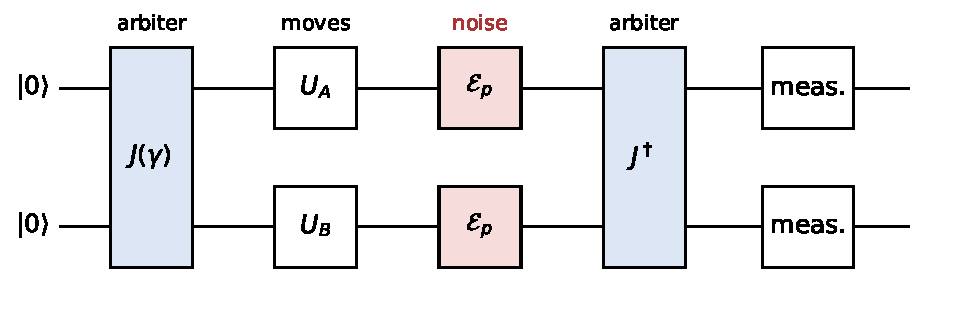
\includegraphics[width=0.8\linewidth]{../figures/ewl_circuit.pdf}
\caption{The EWL protocol as a circuit. The noise channels $\mathcal E_p$ (red) are inserted in \cref{sec:noise} between the players' moves $U_A,U_B$ and the arbiter's gate $J^\dagger$; without them the circuit is the noiseless game of this section.}
\label{fig:circuit}
\end{figure}

\paragraph{Classical embedding.} $C\otimes C$, $C\otimes D$, $D\otimes C$, $D\otimes D$ commute with $D\otimes D$ (and $C=\mathbb I$), hence with $J$. For $M$ one of them, $J^\dagger MJ\ket{00}=M\ket{00}=\pm\ket{xy}$ with $x,y\in\{C,D\}$ the labels of the chosen moves ($D\ket0=-\ket1$ is a global sign). So for classical moves the outcome is the deterministic classical outcome for every $\gamma$.

\subsection{Equilibria in the two-parameter set}\label{sec:equilibria}
\paragraph{Definitions.} A \emph{strategy} of a player is a unitary $U\in U(2)$ (a global phase changes no probability, so $U\sim e^{i\alpha}U$). A \emph{mixed strategy} is a finite probability distribution $\{p_k,U_k\}$; if Bob mixes, the state entering $J^\dagger$ is the corresponding ensemble average, so the expected payoff is the $p$-weighted average of the pure-strategy payoffs, where $\$_A=\sum_x\pi^A_x\Pr(x)$ with $\pi^A=(3,0,5,1)$ and $\pi^B=(3,5,0,1)$ for the outcomes $CC,CD,DC,DD$. A strategy is a \emph{best response} to the opponent's strategy if it maximises the player's expected payoff against it. A profile is a \emph{Nash equilibrium} (NE) if each strategy is a best response to the other; it is \emph{strict} if each is the unique best response and \emph{weak} otherwise. Payoffs are linear in a player's own mixture, so it suffices to test pure deviations. The game is \emph{symmetric}: $\$_B(U_A,U_B)=\$_A(U_B,U_A)$, because $\mathrm{SWAP}\,J\,\mathrm{SWAP}=J$ ($D\otimes D$ is swap-invariant), $\mathrm{SWAP}\ket{00}=\ket{00}$, and $\pi^B$ is $\pi^A$ with the two middle entries exchanged. Hence for a symmetric profile $(\Sigma,\Sigma)$ Bob's deviations pay what Alice's do, and it suffices to check Alice's.

In this subsection both players are restricted to the two-parameter set $U(\theta,\phi)$, $\theta\in[0,\pi]$, $\phi\in[0,\pi/2]$, and every NE statement refers to that set; the full $SU(2)$ case is treated in \cref{sec:fullsu2}. Write $c=\cos\frac\theta2$, $s=\sin\frac\theta2$, so $c^2+s^2=1$ and $c,s\ge0$. Computing $\ket{\psi_f}$ from \cref{eq:U} with $J=\cos\frac\gamma2\,\mathbb{I}+i\sin\frac\gamma2\,D\otimes D$ (derivation in \cref{app:derivation}) gives the following outcome probabilities.

\paragraph{Deviation against $D$.}
\[
P_{CC}=0,\quad P_{CD}=(1-\sin^2\gamma\sin^2\phi)\,c^2,\quad P_{DC}=\sin^2\gamma\sin^2\phi\,c^2,\quad P_{DD}=s^2,
\]
\begin{equation}
\$_A\big(U(\theta,\phi),D\big)=5\sin^2\gamma\,\sin^2\phi\,c^2+s^2\;\le\;5\sin^2\gamma\,c^2+s^2\;\le\;\max(5\sin^2\gamma,\,1).\label{eq:devD}
\end{equation}
The first inequality uses $\sin^2\phi\le1$; the second holds because the middle expression is a convex combination (weights $c^2,s^2$) of $5\sin^2\gamma$ and $1$. The maximum $5\sin^2\gamma$ is attained by $Q$ ($\theta=0,\phi=\pi/2$). Since $\$_A(D,D)=1$,
\[
(D,D)\text{ is a NE}\iff 5\sin^2\gamma\le1\iff\gamma\le\arcsin(1/\sqrt5)\approx0.4636 .
\]

\paragraph{Deviation against $Q$.}
\[
P_{CC}=(1-\sin^2\gamma\cos^2\phi)\,c^2,\quad P_{CD}=\sin^2\gamma\,s^2,\quad P_{DC}=\cos^2\gamma\,s^2,\quad P_{DD}=\sin^2\gamma\cos^2\phi\,c^2,
\]
\begin{equation}\begin{split}
\$_A\big(U(\theta,\phi),Q\big)&=(3-2\sin^2\gamma\cos^2\phi)\,c^2+5\cos^2\gamma\,s^2\\
&\le\;3c^2+5\cos^2\gamma\,s^2\;\le\;\max(3,\,5\cos^2\gamma).\end{split}\label{eq:devQ}
\end{equation}
The maximum $5\cos^2\gamma$ is attained by $D$ ($\theta=\pi$). Since $\$_A(Q,Q)=3$ (set $\theta=0,\phi=\pi/2$),
\[
(Q,Q)\text{ is a NE}\iff 5\cos^2\gamma\le3\iff\sin^2\gamma\ge\tfrac25\iff\gamma\ge\arcsin\sqrt{2/5}\approx0.6847 .
\]
The maximum over the set is exactly $\max(5\cos^2\gamma,3)$ here and $\max(5\sin^2\gamma,1)$ against $D$, so both equivalences are exact; at each threshold the NE is weak because the deviation ties. In the window $\arcsin(1/\sqrt5)<\gamma<\arcsin\sqrt{2/5}$ neither of these two profiles is a NE. At $\gamma=\pi/2$, \cref{eq:devD} gives Alice $5$ for playing $Q$ against $D$, so $(D,D)$ is unstable, while $(Q,Q)$ pays $(3,3)$. Each set of probabilities sums to $c^2+s^2=1$. We cross-checked the expressions symbolically (SymPy, \texttt{verify\_sympy.py}) and the thresholds by a grid search over $41\times21$ deviations (\cref{fig:gamma}).

Du \emph{et al.}~\cite{du} report two entanglement thresholds separating classical, intermediate and quantum regions in this game in a nuclear magnetic resonance (NMR) experiment. All NE statements in this subsection hold only in the two-parameter set, which is not closed under composition: for example $QD=(iZ)(iY)=iX=\begin{pmatrix}0&i\\i&0\end{pmatrix}$ is not of the form \cref{eq:U}, whose off-diagonal entries are $s$ and $-s$ with $s\ge0$ real. This $iX$ is one of the moves used in \cref{sec:fullsu2}.

\begin{figure}[tbp]\centering
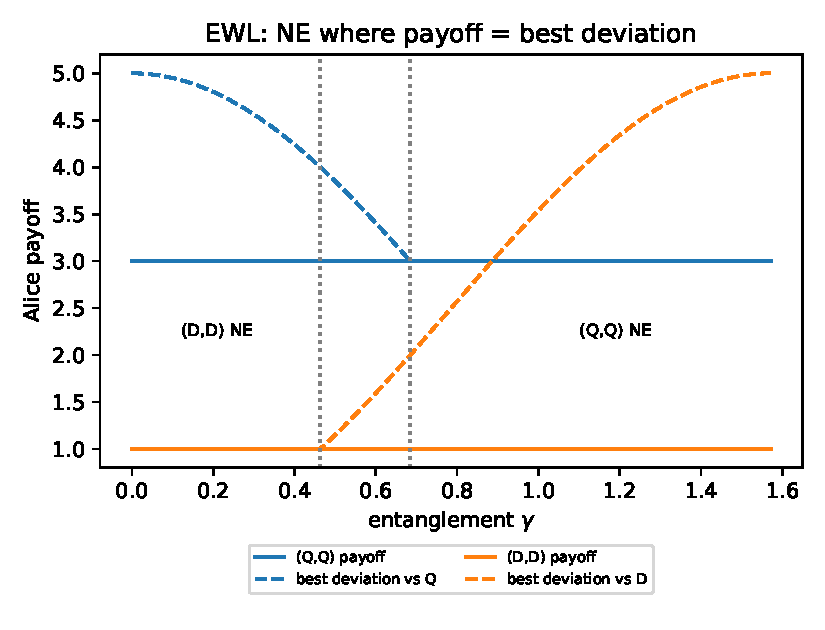
\includegraphics[width=0.6\linewidth]{../figures/ewl_gamma.pdf}
\caption{Noiseless EWL versus entanglement $\gamma$. Solid: payoff of $(Q,Q)$ and $(D,D)$, which do not depend on $\gamma$. Dashed: Alice's best unilateral deviation over the $41\times21$ grid, which contains the profile itself, so dashed $\ge$ solid. A profile is a NE where the dashed curve coincides with its solid line. Each dashed curve leaves its solid line exactly at the analytic thresholds $\arcsin(1/\sqrt5)$ and $\arcsin\sqrt{2/5}$ (dotted), and between them neither profile is an equilibrium.}
\label{fig:gamma}
\end{figure}

\subsection{Full \texorpdfstring{$SU(2)$}{SU(2)}: no pure equilibrium, two mixed ones}\label{sec:fullsu2}
Benjamin and Hayden \cite{bh} showed that at $\gamma=\pi/2$, for any $U_B$ there is a $U_A$ giving Alice $5$ (see also the reply \cite{ewlreply}). A short proof follows.

\textbf{Step 1: rewrite the entangled state.} Let $\ket\Phi=\ket{00}+\ket{11}$ and $P=\mathrm{diag}(1,i)$. Then $J\ket{00}=\tfrac1{\sqrt2}(\mathbb I\otimes P)\ket\Phi$, and for any matrices $(A\otimes B)\ket\Phi=(AB^{T}\otimes\mathbb I)\ket\Phi$.

\textbf{Step 2: the target state.} $J\ket{10}=\tfrac1{\sqrt2}(\ket{10}-i\ket{01})=\tfrac1{\sqrt2}(M\otimes\mathbb I)\ket\Phi$ with $M=\ket1\bra0-i\ket0\bra1$ unitary.

\textbf{Step 3: the counter-move.} Choose
\[
U_A=M\,\overline{U_B}\,P^\dagger\qquad(\text{unitary, with }\overline{U_B}=(U_B^{T})^{-1}).
\]
Then
\[
(U_A\otimes U_B)J\ket{00}=\tfrac1{\sqrt2}(U_AP\,U_B^{T}\otimes\mathbb I)\ket\Phi=\tfrac1{\sqrt2}(M\otimes\mathbb I)\ket\Phi=J\ket{10},
\]
so $\ket{\psi_f}=J^\dagger J\ket{10}=\ket{DC}$ and $\$_A=5$, $\$_B=0$. The global phase of $U_A$ is irrelevant, so $U_A$ may be taken in $SU(2)$; it need not lie in the two-parameter set.

\textbf{Step 4: no pure equilibrium.} Since $5$ is the maximal payoff and, by Step 3, Alice has a deviation earning $5$ against every $U_B$, in a pure NE Alice would have to earn $5$, forcing the outcome $\ket{DC}$ and $\$_B=0$; but by the swap symmetry there is a $U_B'$ giving Bob $5$, so Bob deviates. Hence no pure profile is a NE at $\gamma=\pi/2$. Mixed strategies remain \cite{ew2000}:
\begin{enumerate}
\item \textbf{Mixed NE with payoff 5/2 (at $\gamma=\pi/2$).} Alice plays $\mathbb{I}$ or $-iZ$, Bob plays $D$ or $-iX$, each with probability $1/2$ \cite{ew2000}. The four pairings give $(\mathbb I,D)\to(0,5)$, $(\mathbb I,-iX)\to(5,0)$, $(-iZ,D)\to(5,0)$ and $(-iZ,-iX)\to(0,5)$, so each player expects $5/2$.

\emph{Proof that no deviation pays more than $5/2$.} Let Alice deviate to a general $U_A=\begin{pmatrix}a&b\\-\bar b&\bar a\end{pmatrix}$, $|a|^2+|b|^2=1$, $a=a_1+ia_2$, $b=b_1+ib_2$ (any element of $U(2)$ is a phase times such a matrix). At $\gamma=\pi/2$, $\cos\frac\gamma2=\sin\frac\gamma2=1/\sqrt2$ and \cref{eq:Jd} reads
\[
f_{00}=\tfrac{\alpha_{00}-i\alpha_{11}}{\sqrt2},\quad f_{11}=\tfrac{\alpha_{11}-i\alpha_{00}}{\sqrt2},\quad f_{01}=\tfrac{\alpha_{01}+i\alpha_{10}}{\sqrt2},\quad f_{10}=\tfrac{\alpha_{10}+i\alpha_{01}}{\sqrt2}.
\]

\textbf{Step 1: Alice against $D$.} We have
\[
(U_A\otimes D)J\ket{00}=\tfrac1{\sqrt2}(ib\ket{00}-a\ket{01}+i\bar a\ket{10}+\bar b\ket{11}),
\]
so $(f_{00},f_{01},f_{10},f_{11})=(-b_2,-a_1,a_2,b_1)$, i.e.\ $P_{CC}=b_2^2$, $P_{CD}=a_1^2$, $P_{DC}=a_2^2$, $P_{DD}=b_1^2$ and $\$_A(U_A,D)=3b_2^2+5a_2^2+b_1^2$.

\textbf{Step 2: Alice against $-iX\sim X$} (a global phase does not matter). We have
\[
(U_A\otimes X)J\ket{00}=\tfrac1{\sqrt2}(ib\ket{00}+a\ket{01}+i\bar a\ket{10}-\bar b\ket{11}),
\]
so $(f_{00},f_{01},f_{10},f_{11})=(ib_1,ia_2,ia_1,ib_2)$ and $\$_A(U_A,X)=3b_1^2+5a_1^2+b_2^2$.

\textbf{Step 3: average.} Against Bob's $50/50$ mixture Alice earns the average,
\[
\tfrac12\big[5(a_1^2+a_2^2)+4(b_1^2+b_2^2)\big]=\tfrac52|a|^2+2|b|^2=2+\tfrac12|a|^2\le\tfrac52,
\]
with equality iff $|a|=1$, i.e.\ $U_A$ diagonal. By linearity no mixed deviation does better.

\textbf{Step 4: Bob.} Let $G=\begin{pmatrix}a&b\\-\bar b&\bar a\end{pmatrix}$ answer Alice's mixture $\{\mathbb I,-iZ\}$. From
\[
(\mathbb I\otimes G)J\ket{00}=\tfrac1{\sqrt2}(a\ket{00}-\bar b\ket{01}+ib\ket{10}+i\bar a\ket{11})
\]
one gets $P_{CC}=a_1^2$, $P_{DD}=a_2^2$, $P_{CD}=b_1^2$, $P_{DC}=b_2^2$, so $\$_B=3a_1^2+a_2^2+5b_1^2$. From
\[
(Z\otimes G)J\ket{00}=\tfrac1{\sqrt2}(a\ket{00}-\bar b\ket{01}-ib\ket{10}-i\bar a\ket{11})
\]
one gets $P_{CC}=a_2^2$, $P_{DD}=a_1^2$, $P_{CD}=b_2^2$, $P_{DC}=b_1^2$, so $\$_B=3a_2^2+a_1^2+5b_2^2$. The average is $2|a|^2+\tfrac52|b|^2=2+\tfrac12|b|^2\le\tfrac52$, with equality iff $a=0$. Hence the profile is a NE.

\begingroup\sloppy\textbf{Not strict.} The best-response set of Alice is the diagonal subgroup $\{\mathrm{diag}(e^{i\alpha},e^{-i\alpha})\}$, which contains $\mathbb I$ and $Q=iZ$ and is a proper subset of $SU(2)$, whereas for $R$ below it is all of $SU(2)$. It uses $iX$, which lies outside the two-parameter set.\par\endgroup
\item \textbf{Focal NE, payoff 9/4.} Each player mixes $\{\mathbb{I},iX,iY,iZ\}$ uniformly \cite{ew2000}.
\end{enumerate}

\begin{proposition}\label{prop:focal}
At $\gamma=\pi/2$, let $R$ denote the uniform mixture of $\{\mathbb{I},iX,iY,iZ\}$. If Bob plays $R$, every strategy of Alice yields exactly $9/4$. Hence $(R,R)$ is a weak Nash equilibrium in which every strategy is a best response.
\end{proposition}
\begin{proof}
At $\gamma=\pi/2$, $\ket\Psi=J\ket{00}=(\ket{00}+i\ket{11})/\sqrt2$ has reduced states $\rho_A=\rho_B=\mathbb{I}/2$ (it is maximally entangled). For any unitary $U_A$ the state $\ket{\Psi'}=(U_A\otimes\mathbb{I})\ket\Psi$ has the same marginal on Bob, $\rho_B'=\mathbb{I}/2$, since Alice's local unitary does not touch it. Write $\ket{\sigma_k\Psi'}=(\mathbb{I}\otimes\sigma_k)\ket{\Psi'}$ for $\sigma_k\in\{\mathbb{I},X,Y,Z\}$. Then $\langle\sigma_j\Psi'|\sigma_k\Psi'\rangle=\langle\Psi'|\mathbb{I}\otimes\sigma_j^\dagger\sigma_k|\Psi'\rangle=\tr(\rho_B'\sigma_j\sigma_k)=\tfrac12\tr(\sigma_j\sigma_k)=\delta_{jk}$. So the four vectors are orthonormal in a four-dimensional space, hence an orthonormal basis, and $\sum_k\ket{\sigma_k\Psi'}\bra{\sigma_k\Psi'}=\mathbb{I}_4$ (completeness). Bob's strategies are $\mathbb I$ and $i\sigma_k$ for $k=1,2,3$, so the state entering $J^\dagger$ is
\[
\rho=\tfrac14\sum_k\ket{\sigma_k\Psi'}\bra{\sigma_k\Psi'}=\tfrac14\,\mathbb{I}_4.
\]
The phases $i$ in $iX,iY,iZ$ cancel in the projectors. The measured state is $J^\dagger\rho J=\tfrac14J^\dagger J=\mathbb{I}_4/4$, so every outcome has probability $1/4$ and $\$_A=\tfrac14(3+0+5+1)=9/4$ for every $U_A$. The same holds for mixtures of $U_A$, by linearity. By swap symmetry Bob, facing Alice's $R$, earns $\tfrac14(3+5+0+1)=9/4$ for every $U_B$. So no unilateral deviation changes either payoff, and $(R,R)$ is a NE; it is weak because every strategy is a best response.
\end{proof}
Bolonek-Laso\'n and Kosi\'nski \cite{bolonek} classify the mixed equilibria of the maximally entangled game using Landsburg's method. \Cref{prop:focal} proves directly that $(R,R)$ is an equilibrium in which every strategy is a best response, and our numerics agree (every deviation pays exactly $2.25$); we have not checked how this equilibrium is accounted for in their classification.

\section{Simulation methods}\label{sec:methods}

Most figures and numbers come from \texttt{qgames.py}. The Qiskit cross-checks come from \texttt{qiskit\_circuits.py}, the $SU(2)$ equilibrium checks from \texttt{mixed\_ne.py} and \texttt{focal\_ne.py}, the optimiser and grid-convergence checks from \texttt{refine\_check.py} and \texttt{convergence\_check.py}, the exact noisy EWL results from \texttt{exact\_checks.py}, and the quantum chess results and \cref{fig:chess} from \texttt{chess\_check.py}.
\begin{itemize}
\item \textbf{Exact evolution.} States are evolved as density matrices in numpy. Each channel is a set of Kraus operators, and in the batched deviation search the same channel acts on both qubits as a $16\times16$ superoperator on $\mathrm{vec}(\rho)$, so a whole batch of Alice's candidate moves is evaluated with one matrix product.
\item \textbf{NE test.} A symmetric profile $(\Sigma,\Sigma)$ passes if Alice's best payoff over a $41\times21$ grid of $U(\theta,\phi)$ does not exceed her payoff at $\Sigma$ (tolerance $10^{-9}$). The grid has spacing $\pi/40$ in both $\theta$ and $\phi$ and contains $C$, $D$ and $Q$. To rule out a profitable deviation between grid points, \texttt{refine\_check.py} starts a bounded optimiser (L-BFGS-B on $\theta\in[0,\pi]$, $\phi\in[0,\pi/2]$) from the five best grid points for both $(Q,Q)$ and $(D,D)$ on a sweep of $3\times13\times25\times2=1950$ cases (3 channels, 13 values $p\in[0,0.6]$, 25 values $\gamma\in[0,\pi/2]$, 2 profiles). The optimiser never beats the grid by more than $9\times10^{-16}$ (rounding level) and changes no NE verdict, so the grid results hold over the continuous two-parameter set to optimiser precision. For a symmetric profile $(\Sigma,\Sigma)$ the payoff table, $J$ and the channels are invariant under exchanging the players, so Bob's deviations give the same answer; the asymmetric mixed equilibrium of \cref{sec:fullsu2} was checked for both players.
\item \textbf{Thresholds.} The entanglement threshold $\gamma^*$ at which $(Q,Q)$ becomes a NE is found by bisection on this test over $[0,\pi/2]$ with tolerance $10^{-4}$. Bisection assumes a single transition in $\gamma$, which a 400-point scan in \texttt{convergence\_check.py} confirms for $p=0.1,0.3,0.6$ in all three channels. The CHSH noise thresholds $p^*$ are roots of $S=2$ found with \texttt{scipy.optimize.brentq}.
\item \textbf{CHSH optimum.} $S_{\max}$ for a given noisy state is computed with the Horodecki criterion (\cref{sec:chsh-noise}), so no search over settings is needed.
\item \textbf{Cross-checks.} \texttt{qiskit\_circuits.py} implements both games as Qiskit circuits: 20 random EWL cases agree with the numpy model, and a sampled CHSH run with 100\,000 shots per setting gives $S=2.837\pm0.005$, consistent with $2\sqrt2=2.828$ within two standard errors (seed 1). Both Qiskit checks are noiseless and use ideal statevector simulation; the noisy results are numpy only. The expressions \cref{eq:devD,eq:devQ} were verified symbolically with SymPy (\texttt{verify\_sympy.py}). \texttt{mixed\_ne.py} and \texttt{focal\_ne.py} check the mixed equilibria against Haar-random deviations.
\end{itemize}

\section{Noise: the course channels applied to both games}\label{sec:noise}

\subsection{Model}
We use the channels of the course notes (Topic 9) \cite{notes}, applied independently and identically to both qubits so that both games stay symmetric (the channel $\mathcal E_p\otimes\mathcal E_p$ commutes with $\mathrm{SWAP}$, so the swap argument of \cref{sec:equilibria} still applies and it suffices to check Alice's deviations):
\begin{align*}
\text{depolarizing:}&\quad \rho\mapsto(1-p)\rho+\tfrac p3\textstyle\sum_{i=1}^3\sigma_i\rho\sigma_i\\
&\qquad(\text{Bloch vector}\times(1-\tfrac43p),\ p\in[0,1]),\\
\text{dephasing:}&\quad \rho\mapsto(1-\tfrac p2)\rho+\tfrac p2 Z\rho Z,\\
\text{amplitude damping:}&\quad K_0=\mathrm{diag}(1,\sqrt{1-p}),\ K_1=\sqrt p\,\ket0\bra1.
\end{align*}
All three are CPTP:
\begin{itemize}
\item Depolarizing has Kraus operators $\sqrt{1-p}\,\mathbb I,\sqrt{p/3}\,\sigma_i$ and $(1-p)\mathbb I+3\cdot\frac p3\mathbb I=\mathbb I$.
\item Dephasing has Kraus operators $\sqrt{1-p/2}\,\mathbb I,\sqrt{p/2}\,Z$ and $(1-\frac p2)+\frac p2=1$.
\item For amplitude damping $K_0^\dagger K_0+K_1^\dagger K_1=\mathrm{diag}(1,1-p)+p\ket1\bra1=\mathbb I$ ($\ket1$ decays to $\ket0$); its Bloch action is $(n_1,n_2,n_3)\mapsto(\sqrt{1-p}\,n_1,\sqrt{1-p}\,n_2,(1-p)n_3+p)$.
\end{itemize}
The depolarizing factor follows from $\sum_i\sigma_i\rho\sigma_i=\tfrac12(3\mathbb I-\vec n\cdot\vec\sigma)$.

\begingroup\sloppy In CHSH the noise acts on each qubit of $\ket{\Phi^+}$ before measurement, i.e.\ $\rho=(\mathcal E_p\otimes\mathcal E_p)(\ket{\Phi^+}\!\bra{\Phi^+})$ and
$E_{xy}=\tr[\rho\,A_x\otimes B_y]$; we evaluate both the noiseless optimal settings kept fixed (what a fixed experiment sees) and settings re-optimised for the noisy state. In EWL it acts after the players' moves and before $J^\dagger$ (\cref{fig:circuit}):
\[
\rho_f=J^\dagger\,(\mathcal E_p\otimes\mathcal E_p)\big[(U_A\otimes U_B)J\ket{00}\bra{00}J^\dagger(U_A\otimes U_B)^\dagger\big]\,J .
\]\endgroup

\subsection{CHSH}\label{sec:chsh-noise}
\paragraph{Fixed settings.} Here the noiseless optimal settings are kept and the channel acts on the state. We treat each channel in turn.

\emph{Depolarizing.} Local depolarizing shrinks each Bloch vector by $\eta=1-\tfrac43p$, so all correlators scale by $\eta^2$ (the state has $T=\eta^2\,\mathrm{diag}(1,-1,1)$ and $\langle(\vec a\cdot\vec\sigma)\otimes(\vec b\cdot\vec\sigma)\rangle=\vec a^{\mathsf T}T\vec b$) and $S=2\sqrt2\,\eta^2$. The violation is lost when $\eta^2=1/\sqrt2$, i.e.\ $p^*=\tfrac34(1-2^{-1/4})=0.1193$.

\emph{Dephasing.} Dephasing maps $(n_1,n_2,n_3)\mapsto((1-p)n_1,(1-p)n_2,n_3)$ on each Bloch vector, so it leaves $\langle Z\otimes Z\rangle=1$ intact and scales $\langle X\otimes X\rangle$ to $(1-p)^2$. With the noiseless optimum $A_0=Z$, $A_1=X$, $B_{0,1}=(Z\pm X)/\sqrt2$ (and $\langle Z\otimes X\rangle=0$ preserved), $E_{00}=E_{01}=1/\sqrt2$ come from $\langle Z\otimes Z\rangle$ and $E_{10}=-E_{11}=(1-p)^2/\sqrt2$ from $\langle X\otimes X\rangle$, giving $S=\sqrt2\,[1+(1-p)^2]$ and $p^*=1-\sqrt{\sqrt2-1}=0.3564$.

\emph{Amplitude damping.} The state has $P_{00}=\frac{1+p^2}{2}$, $P_{11}=\frac{(1-p)^2}{2}$, $P_{01}=P_{10}=\frac{p(1-p)}{2}$ and a $\ket{00}\bra{11}$ coherence, so $\langle Z\otimes Z\rangle=(1-p)^2+p^2$, $\langle X\otimes X\rangle=1-p$ and $\langle Z\otimes X\rangle=\langle X\otimes Z\rangle=0$. Hence $E_{00}=E_{01}=\frac{(1-p)^2+p^2}{\sqrt2}$, $E_{10}=-E_{11}=\frac{1-p}{\sqrt2}$ and
\[S=\sqrt2\,\big(2-3p+2p^2\big).\]
$S=2$ reads $2p^2-3p+(2-\sqrt2)=0$, with root $p^*=\tfrac14\big(3-\sqrt{8\sqrt2-7}\big)=0.2308$ in $[0,1]$ (the other root exceeds $1$). This agrees with the numerical root $0.23076$ (\cref{fig:chsh}).

\paragraph{Optimised settings.} A fixed experiment does not have to keep the noiseless settings, so we also ask for the largest value of $S$ over all settings. Let $\rho$ be a two-qubit state, $T_{ij}=\tr[\rho\,\sigma_i\otimes\sigma_j]$ its real $3\times3$ correlation matrix, and $t_1\ge t_2\ge t_3$ the eigenvalues of $T^{\mathsf T}T$. Every $\pm1$ qubit observable is $\pm\mathbb I$ or $\vec a\cdot\vec\sigma$ with $|\vec a|=1$. The Horodecki criterion \cite{horodecki} states that the maximum of $|S|$ over all such observables on each side is
\begin{equation}
S_{\max}=2\sqrt{t_1+t_2},\label{eq:horodecki}
\end{equation}
with $\sigma_1,\sigma_2,\sigma_3=X,Y,Z$, so CHSH can be violated iff $t_1+t_2>1$. The outline of the proof is as follows.
\begin{enumerate}
\item Observables $\pm\mathbb I$ give $|S|\le2$.
\item For $A_0=\vec a\cdot\vec\sigma$, $A_1=\vec a'\cdot\vec\sigma$, $B_0=\vec b\cdot\vec\sigma$, $B_1=\vec b'\cdot\vec\sigma$ (unit vectors) each term is $\vec a^{\mathsf T}T\vec b$ (no local terms occur because all observables are traceless), so
\[
S=\vec a^{\mathsf T}T(\vec b+\vec b')+\vec a'^{\mathsf T}T(\vec b-\vec b').
\]
\item Since $|\vec b|=|\vec b'|=1$, $(\vec b+\vec b')\perp(\vec b-\vec b')$ and $|\vec b+\vec b'|^2+|\vec b-\vec b'|^2=4$, so $\vec b+\vec b'=2\cos\alpha\,\vec c$, $\vec b-\vec b'=2\sin\alpha\,\vec c'$ with orthonormal $\vec c,\vec c'$ and $\alpha\in[0,\pi/2]$.
\item Then, by Cauchy--Schwarz twice,
\[
S=2\cos\alpha\,\vec a^{\mathsf T}T\vec c+2\sin\alpha\,\vec a'^{\mathsf T}T\vec c'\le2\cos\alpha|T\vec c|+2\sin\alpha|T\vec c'|\le2\sqrt{|T\vec c|^2+|T\vec c'|^2}.
\]
\item By the Ky Fan inequality, $|T\vec c|^2+|T\vec c'|^2=\vec c^{\mathsf T}T^{\mathsf T}T\vec c+\vec c'^{\mathsf T}T^{\mathsf T}T\vec c'\le t_1+t_2$.
\item Equality holds for $\vec c,\vec c'$ the top two eigenvectors, $\vec a\propto T\vec c$, $\vec a'\propto T\vec c'$ and $\tan\alpha=|T\vec c'|/|T\vec c|$.
\end{enumerate}
We use \cref{eq:horodecki} as a cited result.

Applying it to $\ket{\Phi^+}$ after the local channels gives the following.
\begin{itemize}
\item \emph{Depolarizing.} $T=\eta^2\,\mathrm{diag}(1,-1,1)$ with $\eta=1-\tfrac43p$ (the state is the Werner state $\eta^2\Phi^++(1-\eta^2)\mathbb I/4$), so $S_{\max}=2\sqrt2\,\eta^2$ coincides with the fixed-setting value and $p^*=0.1193$.
\item \emph{Amplitude damping.} The state is $Z$-diagonal plus a $\ket{00}\bra{11}$ coherence, so $T$ is diagonal: $T_{33}=\langle Z\otimes Z\rangle=(1-p)^2+p^2$, and $T_{11}=-T_{22}=1-p$ because the coherence is multiplied by $\sqrt{1-p}\cdot\sqrt{1-p}$ (only $K_0\otimes K_0$ preserves it). Thus $T=\mathrm{diag}\big(1-p,\,-(1-p),\,(1-p)^2+p^2\big)$. Since $(1-p)^2+p^2\le1-p\iff p\le\tfrac12$, for $p\le\tfrac12$ the two largest singular values are both $1-p$, so $S_{\max}=2\sqrt2\,(1-p)$ and the violation is lost at $p^*=1-1/\sqrt2=0.2929<\tfrac12$, later than the fixed-setting value $0.2308$. For $p>\tfrac12$, $t_1+t_2=((1-p)^2+p^2)^2+(1-p)^2\le2-4p+3p^2<1$ for $\tfrac13<p<1$ (using $(1-p)^2+p^2\le1$), so $S_{\max}<2$ and the violation does not return.
\item \emph{Dephasing.} $T=\mathrm{diag}\big((1-p)^2,\,-(1-p)^2,\,1\big)$, so $S_{\max}=2\sqrt{1+(1-p)^4}>2$ for every $p<1$. With optimised settings the violation is never lost before the channel fully dephases, although the margin $S_{\max}-2=\frac{2(1-p)^4}{1+\sqrt{1+(1-p)^4}}=(1-p)^4+O((1-p)^8)$ becomes tiny (for example $S_{\max}=2.0001$ at $p=0.9$).
\end{itemize}
The optimised thresholds are our headline values; the fixed-setting thresholds ($0.1193$ depolarizing, $0.2308$ amplitude damping, $0.3564$ dephasing) are what a fixed noiseless-optimal experiment sees.

\begin{figure}[htbp]\centering
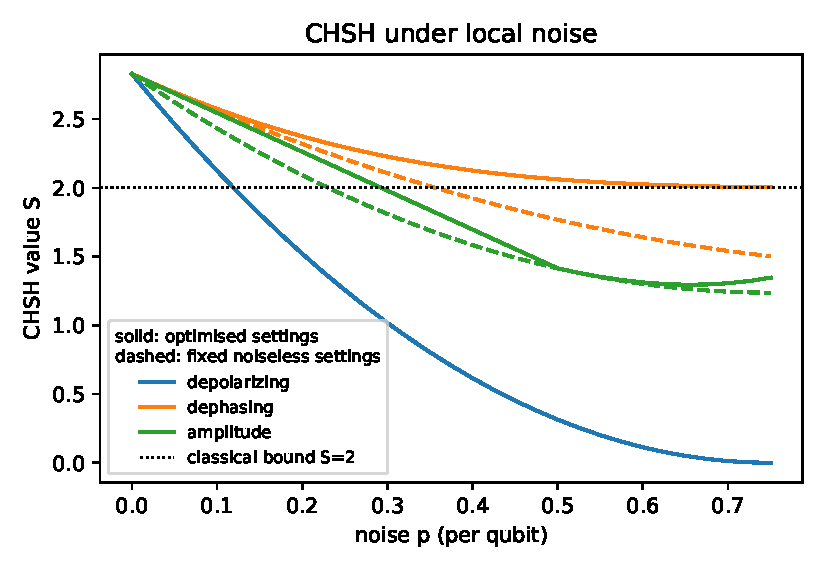
\includegraphics[width=0.7\linewidth]{../figures/chsh_noise.pdf}
\caption{CHSH value under the three channels. Solid: settings optimised for the noisy state; dashed: fixed noiseless settings. With optimised settings the violation ($S>2$) is lost at $p^*=0.119$ (depolarizing) and $0.293$ (amplitude damping) and never under dephasing for $p<1$ (analytically; the plot stops at $p=0.75$). The two depolarizing curves coincide. With fixed settings the thresholds are $0.119$, $0.231$ and $0.356$ for depolarizing, amplitude damping and dephasing.}
\label{fig:chsh}
\end{figure}

\subsection{EWL}
\Cref{fig:phase} shows, over the $(\gamma,p)$ plane, the payoff of $(Q,Q)$ and the boundary of the region where it is a NE in the two-parameter set. \Cref{tab:ewl} lists the entanglement threshold $\gamma^*$ and the payoffs at $\gamma=\pi/2$ for $p=0.1$ and $p=0.3$ only; the phase figure covers $p$ up to $0.6$. The column $\$(D,D)$ is the payoff of the classical profile in the same noisy device, that is, what players earn without using the quantum move.

The thresholds in \cref{tab:ewl} come from bisection on a $41\times21$ deviation grid with bisection tolerance $10^{-4}$ and carry an uncertainty of $\pm0.001$. \texttt{convergence\_check.py} recomputes them on $121\times61$ and $401\times201$ grids (agreement to $10^{-4}$), confirms a single switch from non-NE to NE along a 400-point $\gamma$ scan for $p=0.1,0.3,0.6$ in all three channels, and runs the continuous optimiser just above each $\gamma^*$, where it finds no profitable deviation. It also gives the dephasing value $p\approx0.622$ and the amplitude-damping threshold $0.671$ at $p=0.6$ quoted below.
\begin{table}[htbp]\centering\small
\caption{EWL $(Q,Q)$ equilibrium threshold $\gamma^*$ and payoffs at $\gamma=\pi/2$. The row $p=0$ is analytic; the numerical accuracy of the thresholds is described in the text.}
\label{tab:ewl}
\begin{tabular}{lccccccc}
\toprule
channel & \multicolumn{3}{c}{$p=0.1$} & \multicolumn{3}{c}{$p=0.3$}\\
\cmidrule(lr){2-4}\cmidrule(lr){5-7}
 & $\gamma^*$ & $\$(Q,Q)$ & $\$(D,D)$ & $\gamma^*$ & $\$(Q,Q)$ & $\$(D,D)$\\
\midrule
none ($p=0$) & 0.685 & 3.000 & 1.000 & 0.685 & 3.000 & 1.000\\
depolarizing & 0.712 & 2.813 & 1.311 & 0.785 & 2.520 & 1.800\\
dephasing & 0.747 & 2.810 & 1.190 & 0.909 & 2.490 & 1.510\\
amplitude damping & 0.682 & 2.945 & 1.145 & 0.678 & 2.805 & 1.405\\
\bottomrule
\end{tabular}
\end{table}
Depolarizing and dephasing noise push the threshold to larger $\gamma$: more entanglement is needed for the quantum equilibrium to exist, and it pays less. Amplitude damping moves the threshold slightly down ($0.678<0.685$ at $p=0.3$). The equilibrium payoff $\$(Q,Q)$ stays above the noisy $\$(D,D)$ in every tested case (for dephasing above $p\approx0.423$ this compares with a profile that is no longer a classical equilibrium, see below), but the margin shrinks as noise grows because noise also raises the $(D,D)$ payoff. \Cref{fig:adv} (right) shows this margin at $\gamma=\pi/2$ for $p\le0.6$: it falls to $0.080$ for depolarizing noise, $0.320$ for dephasing and $0.800$ for amplitude damping, and $(Q,Q)$ is still an equilibrium at $\gamma=\pi/2$ at $p=0.6$ for all three channels. Whether $(D,D)$ is the right classical baseline is examined below. Beyond the plotted range, under dephasing $(Q,Q)$ stops being a NE at $\gamma=\pi/2$ at $p=1-1/\sqrt7\approx0.622$ (proved below), and under depolarizing noise the margin reaches $0$ at $p=3/4$, where every profile pays $9/4$. This last fact is exact. At $p=3/4$ the depolarizing map is $\rho\mapsto\frac14\sum_{\mu=0}^{3}\sigma_\mu\rho\sigma_\mu=\tr(\rho)\,\mathbb I/2$ for every single-qubit $\rho$, and since product operators $\sigma\otimes\tau$ span all two-qubit operators and both sides are linear, $(\mathcal E_{3/4}\otimes\mathcal E_{3/4})(\rho)=\tr(\rho)\,\mathbb I/4$ for every two-qubit $\rho$. Then $\rho_f=J^\dagger(\mathbb I/4)J=\mathbb I/4$ whatever $U_A,U_B$ are, each outcome has probability $1/4$, and each player gets $\frac14(3+0+5+1)=9/4$. Every profile is then a weak NE and no strategy carries any advantage. Equivalently, the Bloch shrink factor $1-\frac43p$ is $0$ at $p=3/4$.

\paragraph{Exact dephasing threshold at $\gamma=\pi/2$.} Let $k=(1-p)^2$, the factor by which local dephasing on both qubits multiplies the off-diagonal elements $\ket{00}\!\bra{11}$ and $\ket{01}\!\bra{10}$. Against $Q$, Alice's payoff for $U(\theta,\phi)$ is
\begin{equation}
\$_A\big(U(\theta,\phi),Q\big)=\tfrac52(1-k)+\cos^2\tfrac\theta2\Big[2k\sin^2\phi+\tfrac{3k-1}2\Big].\label{eq:dephQ}
\end{equation}
At $k=1$ this reduces to the noiseless \cref{eq:devQ} at $\gamma=\pi/2$. The bracket is largest at $\sin^2\phi=1$, where it equals $(7k-1)/2$, and the payoff is linear in $\cos^2\frac\theta2\in[0,1]$. So the best deviation is $Q$ itself ($\theta=0,\phi=\pi/2$, payoff $2+k$) when $7k\ge1$ and $D$ ($\theta=\pi$, payoff $\frac52(1-k)$) when $7k<1$. Hence $(Q,Q)$ is a NE in the two-parameter set iff $(1-p)^2\ge1/7$, i.e.\ $p\le1-1/\sqrt7=0.62204$, in agreement with the bisection value $0.6220$. \texttt{exact\_checks.py} evaluates the density-matrix evolution symbolically and checks \cref{eq:dephQ} against it at 40 random points $(\theta,\phi,p)$.

\paragraph{A classical baseline that is itself an equilibrium.} The margin $\$(Q,Q)-\$(D,D)$ compares the quantum equilibrium with $(D,D)$, which is the right baseline only while $(D,D)$ is an equilibrium of the classical game that the same noisy device induces when both players may use only $C$ and $D$ (no other unitaries). Write $\pi_{CC},\pi_{CD},\pi_{DC},\pi_{DD}$ for Alice's payoffs at the four profiles at $\gamma=\pi/2$; Bob's payoffs follow by symmetry. In this $2\times2$ game $(D,D)$ is a NE iff $\pi_{DD}\ge \pi_{CD}$, $(C,C)$ is a NE iff $\pi_{CC}\ge \pi_{DC}$, and $(C,D)$ is a NE iff $\pi_{CD}\ge \pi_{DD}$ (Alice) and $\pi_{DC}\ge \pi_{CC}$ (Bob). Exact evaluation (\texttt{exact\_checks.py}, symbolic in $p$) gives
\[
\begin{array}{lcc}
 & \pi_{DC}-\pi_{CC} & \pi_{DD}-\pi_{CD}\\[2pt]
\text{depolarizing} & \frac29(4p-3)^2 & \frac19(4p-3)^2\\[2pt]
\text{dephasing} & \frac12(3k+1) & \frac12(3k-1)\\[2pt]
\text{amplitude damping} & \frac12(1-p)(4-p) & \frac12(1-p)(2+p)
\end{array}
\]
For depolarizing noise and amplitude damping both differences are $\ge0$ for every $p\in[0,1]$, so $D$ weakly dominates $C$, $(D,D)$ is a classical equilibrium, and the margin in \cref{fig:adv} is the right comparison. Under dephasing $\pi_{DC}>\pi_{CC}$ always, but $\pi_{DD}<\pi_{CD}$ once $k<1/3$, i.e.\ $p>1-1/\sqrt3\approx0.423$. Above that value $(D,D)$ is no longer a classical equilibrium. The classical game then has the asymmetric equilibria $(C,D)$ and $(D,C)$ and a symmetric mixed equilibrium. Under dephasing the four payoffs are $\pi_{CC}=2+k$ (equal to $\$(Q,Q)$), $\pi_{CD}=\frac52(1-k)$, $\pi_{DC}=\frac52(1+k)$ and $\pi_{DD}=2-k$. Since $\pi_{CD}+\pi_{DC}=5$, the asymmetric equilibria have average payoff $5/2$. In the symmetric mixed equilibrium each player plays $C$ with the probability $q$ that makes the other indifferent between $C$ and $D$, $q=(\pi_{DD}-\pi_{CD})/(\pi_{CC}-\pi_{CD}-\pi_{DC}+\pi_{DD})=(1-3k)/2$, and the payoff is
\[
\$_{\rm mix}=q\pi_{CC}+(1-q)\pi_{CD},\qquad \$(Q,Q)-\$_{\rm mix}=\tfrac14(7k-1)(1+3k).
\]
So $(Q,Q)$ beats the symmetric classical equilibrium exactly when $7k\ge1$, i.e.\ exactly where $(Q,Q)$ is itself an equilibrium ($p\le1-1/\sqrt7$). At $p=0.6$ ($k=0.16$): $q=0.26$, $\$_{\rm mix}=2.1156$ and $\$(Q,Q)=2.16$, a margin of $0.044$. For $0.423<p\le0.622$ the quantum equilibrium therefore beats the symmetric classical equilibrium but pays less than the average $5/2$ of the asymmetric ones. Which classical equilibrium players would reach is a question of equilibrium selection that we do not settle; the positive dephasing margin over $(D,D)$ in \cref{fig:adv} above $p\approx0.423$ should be read with this caveat.

\begin{figure}[tbp]\centering
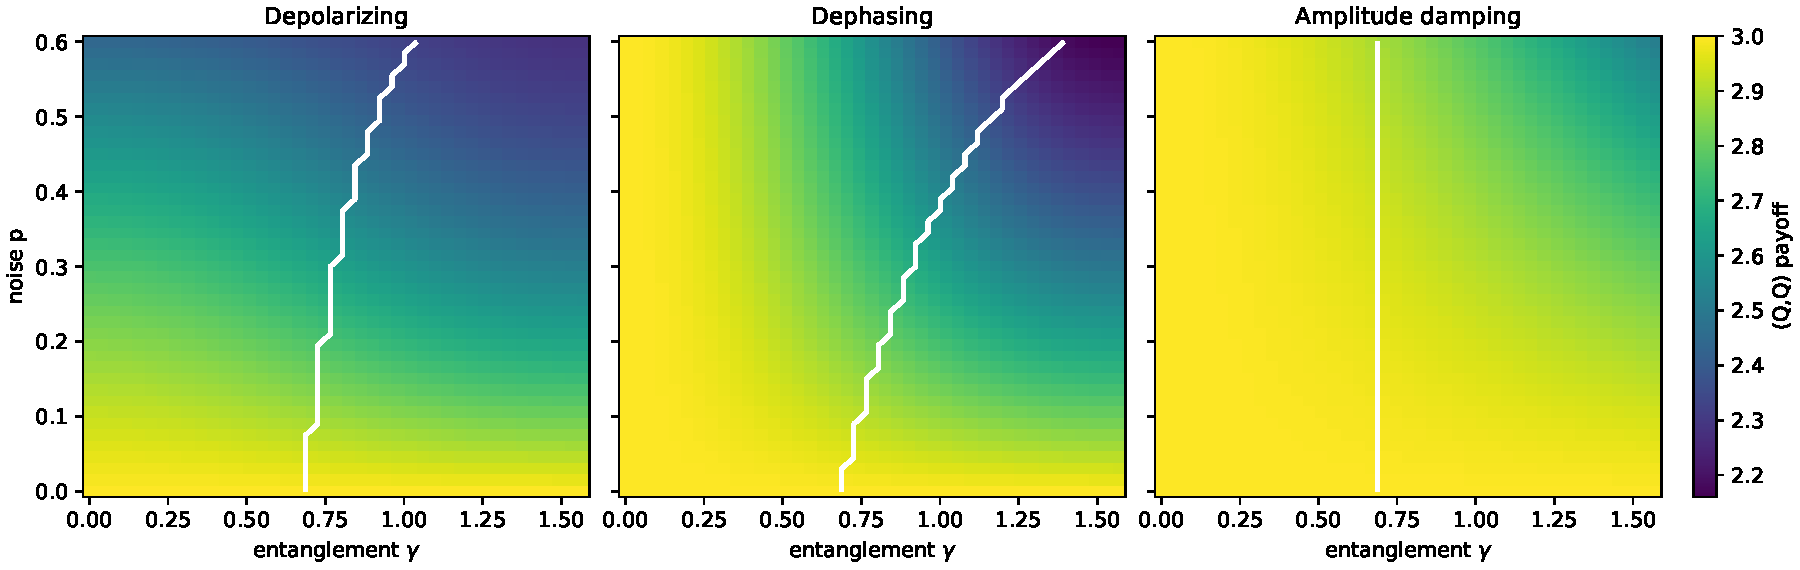
\includegraphics[width=\linewidth]{../figures/ewl_phase.pdf}
\caption{EWL $(Q,Q)$ payoff (colour, one shared scale) and the boundary (white) to the right of which $(Q,Q)$ is a NE in the two-parameter set. Depolarizing and dephasing noise move the boundary to larger $\gamma$, dephasing much more strongly, and all three channels lower the payoff. Amplitude damping moves the boundary only slightly, to lower $\gamma$ (from $0.685$ to $0.671$ at $p=0.6$). Left of the boundary the colour is \emph{not} an equilibrium payoff.}
\label{fig:phase}
\end{figure}

\begin{figure}[tbp]\centering
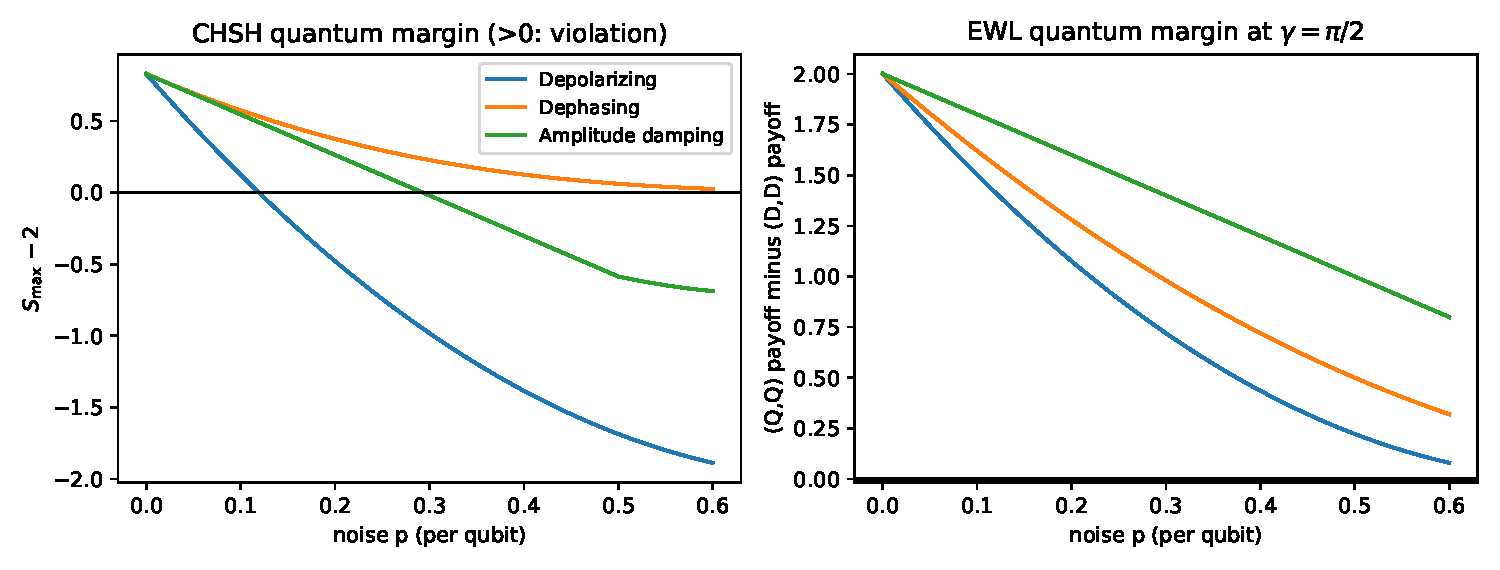
\includegraphics[width=\linewidth]{../figures/advantage_vs_noise.pdf}
\caption{Quantum margins as a function of noise with maximally entangled resources ($\ket{\Phi^+}$ for CHSH, $\gamma=\pi/2$ for EWL). Left: CHSH value above the classical bound with optimised settings, $S_{\max}-2$. Right: EWL payoff of $(Q,Q)$ minus the noisy payoff of $(D,D)$ at $\gamma=\pi/2$. The CHSH margin crosses zero for depolarizing and amplitude damping noise and decays towards zero for dephasing ($0.025$ at $p=0.6$), whereas the EWL margin remains positive for all three channels over the plotted range $p\le0.6$. Under dephasing above $p\approx0.423$, $(D,D)$ is no longer a classical equilibrium, so there the right panel compares with a non-equilibrium profile (see text). The two vertical scales are not commensurable; only signs and zero crossings are compared.}
\label{fig:adv}
\end{figure}

\section{A third case: split and merge in quantum chess}\label{sec:chess}
Quantum chess \cite{cantwell,qchess} adds quantum moves to chess. We study only its basic move pair: a piece is split over two squares and later merged back. This case has no equilibrium and no Bell inequality; the quantum feature it uses is coherence between the two branches of one piece. We prove how often the merge returns the piece, compare with a classical random move, and apply the three channels of \cref{sec:noise}.

\subsection{Rules and encoding}
Each square is a qubit, $\ket1$ for occupied and $\ket0$ for empty. We use three squares, a source $s$ and targets $a,b$, ordered $(s,a,b)$. Following Cantwell \cite{cantwell,qchess}, a jump between two squares is the gate $W$ (iSWAP) and a split uses its square root $V$:
\[
W=\begin{pmatrix}1&0&0&0\\0&0&i&0\\0&i&0&0\\0&0&0&1\end{pmatrix},\qquad
V=\begin{pmatrix}1&0&0&0\\0&\frac1{\sqrt2}&\frac i{\sqrt2}&0\\0&\frac i{\sqrt2}&\frac1{\sqrt2}&0\\0&0&0&1\end{pmatrix},\qquad V^2=W .
\]
Both are unitary and conserve the number of occupied squares. The split is $W_{sb}V_{sa}$ (right factor first) and the merge is $\mathcal M=V_{sa}W_{sb}$. A \emph{classical random move} puts the piece on $a$ or $b$ with probability $1/2$ each, with no phase between the two possibilities. We call the piece \emph{recovered} if, after the merge, the board is exactly $\ket{100}$. \Cref{fig:chesscirc} shows the moves on a board and as a circuit.

\begin{figure}[htbp]\centering
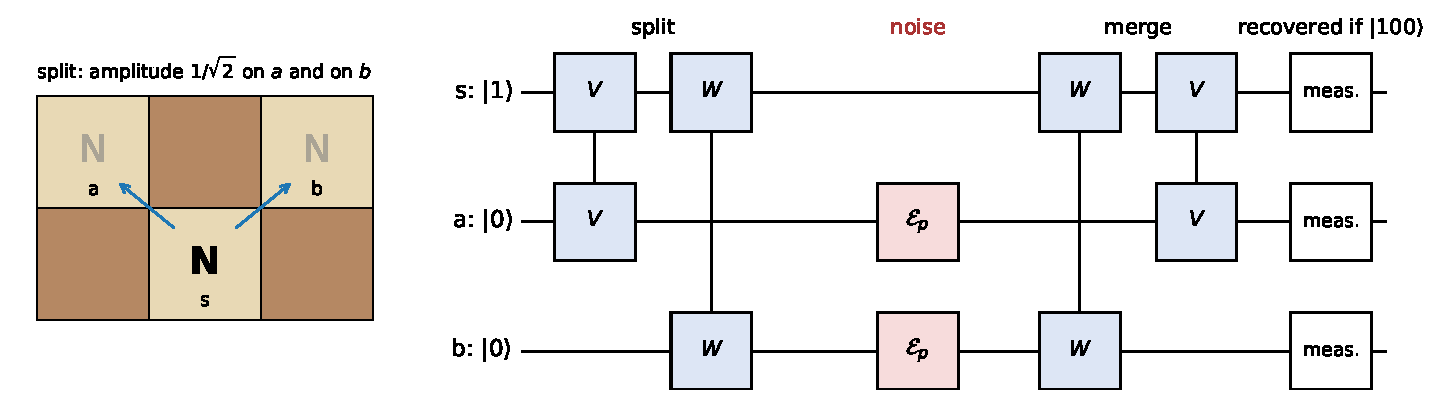
\includegraphics[width=\linewidth]{../figures/chess_circuit.pdf}
\caption{Left: a knight on $s$ is split over $a$ and $b$, each with amplitude $1/\sqrt2$; the grey knights are one piece in superposition, not two pieces. Right: the same move as a circuit on the occupancy qubits $(s,a,b)$. The split is $V$ on $(s,a)$ then $W$ on $(s,b)$; the noise $\mathcal E_p$ acts on the two target squares; the merge applies $W$ then $V$; the piece is recovered if the measured board is $\ket{100}$.}
\label{fig:chesscirc}
\end{figure}

\subsection{Split, merge and the classical comparison}
$V_{sa}\ket{100}=(\ket{100}+i\ket{010})/\sqrt2$, and $W_{sb}$ maps $\ket{100}\to i\ket{001}$ and leaves $\ket{010}$ unchanged, so the split gives
\begin{equation}
\ket\psi=\tfrac{i}{\sqrt2}\big(\ket{001}+\ket{010}\big)=\ket0_s\otimes i\ket{\Psi^+}_{ab},\qquad \ket{\Psi^+}=\tfrac1{\sqrt2}(\ket{01}+\ket{10}),\label{eq:split}
\end{equation}
one piece on $a$ or $b$ with probability $1/2$ each. Applying the merge, $W_{sb}\ket\psi=\tfrac{i}{\sqrt2}(i\ket{100}+\ket{010})$, and then $V_{sa}$ gives $\tfrac{i}{2}\big[i(\ket{100}+i\ket{010})+(i\ket{100}+\ket{010})\big]=-\ket{100}$. The orthogonal state $\ket{\psi_\perp}=\tfrac{i}{\sqrt2}(\ket{001}-\ket{010})$, with the same square probabilities, is sent by the same steps to $-i\ket{010}$.

\begin{proposition}\label{prop:recovery}
For any board state $\rho$, the probability that the merge recovers the piece is $P_{\rm rec}(\rho)=\bra\psi\rho\ket\psi$. If the source is empty, $\rho=\ket0\!\bra0_s\otimes\rho_{ab}$, this is $\bra{\Psi^+}\rho_{ab}\ket{\Psi^+}$. In particular the coherent split is recovered with probability $1$ and the classical random move with probability $1/2$.
\end{proposition}
\begin{proof}
Since $\mathcal M\ket\psi=-\ket{100}$ and $\mathcal M$ is unitary, $\mathcal M^\dagger\ket{100}=-\ket\psi$. Hence $P_{\rm rec}(\rho)=\bra{100}\mathcal M\rho\mathcal M^\dagger\ket{100}=\bra\psi\rho\ket\psi$, and \cref{eq:split} gives the second form. For the coherent split $\rho=\ket\psi\!\bra\psi$ and $P_{\rm rec}=1$. The classical move is $\rho_c=\frac12(\ket{001}\!\bra{001}+\ket{010}\!\bra{010})=\frac12(\ket\psi\!\bra\psi+\ket{\psi_\perp}\!\bra{\psi_\perp})$, so $P_{\rm rec}(\rho_c)=\frac12$.
\end{proof}

The comparison is for a fixed merge operation. A classical rule that simply moved the piece back would also succeed with certainty, so this is not a claim about better chess play: the merge acts as a test that tells a coherent split from a random placement with the same square probabilities.

\subsection{Noise between the moves}
We model the board as stored on the qubits of a quantum computer, as in Cantwell's implementation \cite{cantwell}, and apply the same single-qubit channel $\mathcal E_p$ (\cref{sec:noise}) to the two target squares, the squares that hold the piece while it waits between split and merge. We leave the empty source noiseless; this is a modelling choice, and noise on the source would only add further ways to fail. The channels then have a direct board meaning. Dephasing never changes the occupation of a square and destroys only the phase between the two branches. Amplitude damping $\ket1\to\ket0$ is loss of the piece. Depolarizing noise can also create a piece on an empty square, which the rules of chess forbid; in the hardware model this is a device error. Any board other than $\ket{100}$ after the merge counts as a failed recovery. The classical move $\rho_c$ is exposed to the same noise, and the gates themselves are taken as ideal.

\begin{proposition}\label{prop:chessnoise}
With $\eta=1-\frac43p$, $v=\eta^2$ and $k=(1-p)^2$, the recovery probabilities of the coherent split ($P_q$) and of the classical random move ($P_c$) are
\[
\begin{array}{lccc}
 & P_q & P_c & P_q-P_c\\[2pt]
\text{depolarizing} & \frac14(1+3v) & \frac14(1+v) & \frac v2\\[2pt]
\text{dephasing} & \frac12(1+k) & \frac12 & \frac k2\\[2pt]
\text{amplitude damping} & 1-p & \frac12(1-p) & \frac12(1-p)
\end{array}
\]
for $p\in[0,1]$. In every case $P_q-P_c=\mathrm{Re}\bra{01}\rho_{ab}\ket{10}$, the coherence between the two branches that survives the noise.
\end{proposition}
\begin{proof}
By \cref{prop:recovery} we need $\bra{\Psi^+}\rho_{ab}\ket{\Psi^+}$ for $\rho_{ab}=(\mathcal E_p\otimes\mathcal E_p)(\ket{\Psi^+}\!\bra{\Psi^+})$ and for $\rho_{ab}=(\mathcal E_p\otimes\mathcal E_p)(\rho_c)$, where now $\rho_c=\frac12(\ket{01}\!\bra{01}+\ket{10}\!\bra{10})$. Note $\bra{\Psi^+}\rho_c\ket{\Psi^+}=\frac12$.

\textbf{Depolarizing.} One qubit: $\mathcal E_p(X)=\eta X+(1-\eta)\tr(X)\,\mathbb I/2$ (the Bloch shrink of \cref{sec:noise}). On two qubits, $(\mathcal E_p\otimes\mathcal E_p)(\rho)=\eta^2\rho+\eta(1-\eta)\big(\rho_a\otimes\frac{\mathbb I}2+\frac{\mathbb I}2\otimes\rho_b\big)+(1-\eta)^2\frac{\mathbb I}4$. Both states have marginals $\rho_a=\rho_b=\mathbb I/2$, so each becomes $v\rho+(1-v)\mathbb I/4$. With $\bra{\Psi^+}\mathbb I/4\ket{\Psi^+}=\frac14$: $P_q=v+\frac{1-v}4$ and $P_c=\frac v2+\frac{1-v}4$.

\textbf{Dephasing.} Each qubit's off-diagonal elements are multiplied by $1-p$ and its diagonal is unchanged. In $\ket{\Psi^+}\!\bra{\Psi^+}=\frac12(\ket{01}\!\bra{01}+\ket{10}\!\bra{10}+\ket{01}\!\bra{10}+\ket{10}\!\bra{01})$ the cross terms differ on both qubits and are multiplied by $k$; so $P_q=\frac12(1+k)$. $\rho_c$ is diagonal and unchanged, $P_c=\frac12$.

\textbf{Amplitude damping.} With $K_0\ket0=\ket0$, $K_0\ket1=\sqrt{1-p}\ket1$, $K_1\ket1=\sqrt p\ket0$, $K_1\ket0=0$: $(K_0\otimes K_0)\ket{\Psi^+}=\sqrt{1-p}\ket{\Psi^+}$, $(K_1\otimes K_0)\ket{\Psi^+}=(K_0\otimes K_1)\ket{\Psi^+}=\sqrt{p/2}\ket{00}$ and $(K_1\otimes K_1)\ket{\Psi^+}=0$. Summing the four terms, $\rho_{ab}=(1-p)\ket{\Psi^+}\!\bra{\Psi^+}+p\ket{00}\!\bra{00}$, and in the same way $\rho_c\mapsto(1-p)\rho_c+p\ket{00}\!\bra{00}$. Since $\braket{\Psi^+|00}=0$, $P_q=1-p$ and $P_c=\frac12(1-p)$.

\textbf{Margin.} For any $\rho_{ab}$, $\bra{\Psi^+}\rho_{ab}\ket{\Psi^+}=\frac12(\rho_{01,01}+\rho_{10,10})+\mathrm{Re}\,\rho_{01,10}$. In all three cases the noisy coherent and classical states have the same diagonal, and the classical one has $\rho_{01,10}=0$, so the difference is $\mathrm{Re}\,\rho_{01,10}$: $v/2$, $k/2$ and $(1-p)/2$.
\end{proof}

\begin{table}[htbp]\centering\small
\caption{Quantum chess recovery probabilities from \cref{prop:chessnoise}: coherent split $P_q$, classical random move $P_c$, and the negativity $\mathcal N$ of the two target squares after noise.}
\label{tab:chess}
\begin{tabular}{lcccccc}
\toprule
channel & \multicolumn{3}{c}{$p=0.3$} & \multicolumn{3}{c}{$p=0.6$}\\
\cmidrule(lr){2-4}\cmidrule(lr){5-7}
 & $P_q$ & $P_c$ & $\mathcal N$ & $P_q$ & $P_c$ & $\mathcal N$\\
\midrule
depolarizing & 0.520 & 0.340 & 0.020 & 0.280 & 0.260 & 0\\
dephasing & 0.745 & 0.500 & 0.245 & 0.580 & 0.500 & 0.080\\
amplitude damping & 0.700 & 0.350 & 0.231 & 0.400 & 0.200 & 0.061\\
\bottomrule
\end{tabular}
\end{table}

\begin{figure}[htbp]\centering
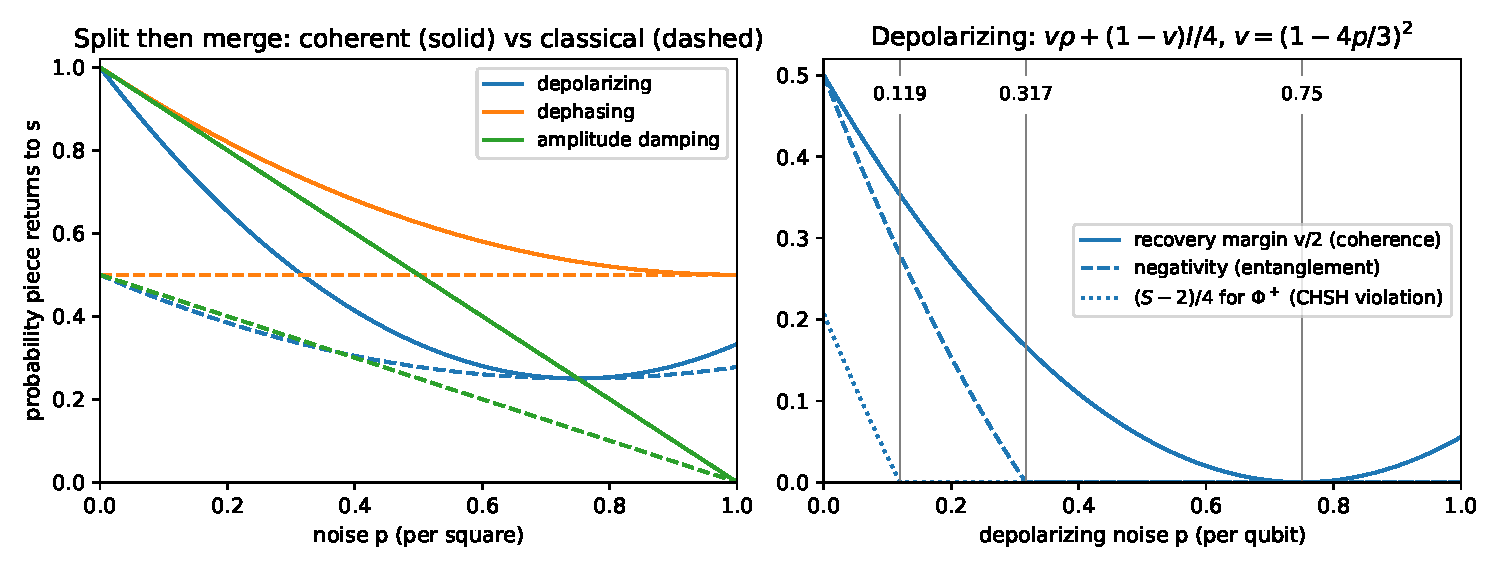
\includegraphics[width=\linewidth]{../figures/chess_noise.pdf}
\caption{Quantum chess under the course channels. Left: probability that the merge returns the piece, for the coherent split (solid) and a classical random move (dashed). The coherent split does better for every $p<1$, except under depolarizing noise at $p=3/4$, where both give $1/4$. Right: depolarizing noise, which maps both $\ket{\Psi^+}$ and $\ket{\Phi^+}$ to $v\rho+(1-v)\mathbb I/4$. The chess recovery margin $v/2$ is zero only at $p=3/4$ (and small but positive beyond it), the negativity of the target pair is zero from $p=0.317$, and the CHSH violation of $\ket{\Phi^+}$, plotted as $(S-2)/4$, is zero from $p=0.119$; only the zeros of the three curves are compared.}
\label{fig:chess}
\end{figure}

\subsection{Coherence, entanglement and nonlocality}
In occupation-number language the split leaves the two target squares in $\ket{\Psi^+}$, an entangled state. For the noisy states the negativity $\mathcal N$ (sum of the moduli of the negative eigenvalues of the partial transpose) is
\[
\mathcal N=\max\big(0,\tfrac{3v-1}4\big),\qquad \tfrac k2,\qquad \tfrac12\Big(\sqrt{p^2+(1-p)^2}-p\Big)
\]
for depolarizing noise, dephasing and amplitude damping. For depolarizing noise the partial transpose of $v\ket{\Psi^+}\!\bra{\Psi^+}+(1-v)\mathbb I/4$ has eigenvalues $\frac{1+v}4$ (three times) and $\frac{1-3v}4$. Under dephasing it has eigenvalues $\frac12,\frac12,\pm\frac k2$. Under amplitude damping its $\{\ket{00},\ket{11}\}$ block is $\begin{pmatrix}p&(1-p)/2\\(1-p)/2&0\end{pmatrix}$, with eigenvalues $\frac12\big(p\pm\sqrt{p^2+(1-p)^2}\big)$. This is single-particle (mode) entanglement, whose status as a resource is debated \cite{vanenk-single}, so we attribute the recovery advantage to coherence.

Depolarizing noise separates the two notions. The target pair is entangled only while $v>1/3$, i.e.\ $p<\frac34(1-1/\sqrt3)=0.317$, but the recovery margin $v/2$ is positive for every $p\ne3/4$: for $0.317<p<3/4$ the merge still tells the coherent split from the classical move although the two squares are no longer entangled. The CHSH state of \cref{sec:chsh-noise} is related to $\ket{\Psi^+}$ by $X$ on one qubit, and local depolarizing noise commutes with local unitaries, so it is depolarized in the same way, $\ket{\Phi^+}\!\bra{\Phi^+}\mapsto v\ket{\Phi^+}\!\bra{\Phi^+}+(1-v)\mathbb I/4$; with settings rotated accordingly the two states have the same CHSH value. Its CHSH violation is lost already at $v=1/\sqrt2$, $p=0.119$. These are the known thresholds of the Werner family \cite{werner}, here read off along one noise parameter: CHSH violation for $p<0.119$, entanglement for $p<0.317$ and a nonzero recovery margin for all $p\ne3/4$ (\cref{fig:chess}, right). The other two channels never remove the recovery margin before $p=1$.

\texttt{chess\_check.py} builds the gates, checks \cref{eq:split}, the merge, \cref{prop:recovery} on random states, and \cref{prop:chessnoise} and the negativities for all three channels at 101 values of $p\in[0,1]$, using the same density-matrix model as the other games. It also runs the noiseless split and merge with Qiskit's \texttt{iSwapGate} and its square root and checks that the outcome probabilities agree.

\section{Discussion}

\paragraph{Kinds of advantage.} The CHSH advantage is a winning probability that no local hidden-variable strategy can reach; in an experiment that closes the locality and detection loopholes it is certified by violation of a Bell inequality, and, for depolarizing and amplitude-damping noise, disappears at a sharp noise threshold. The EWL ``advantage'' is a property of an equilibrium in a game whose rules include the arbiter's gate $J$. Van Enk and Pike \cite{vanenk} and Landsburg \cite{landsburg} argue that the EWL outcomes can be reproduced by a classical game with a suitably enlarged strategy and payoff table; on that view the quantumness lies in the arbiter's apparatus, and the players' moves are ordinary choices in an enlarged classical game.

\paragraph{The threshold depends on the settings and the channel.} Under depolarizing noise the state is Werner-type and the noisy state is the Werner state $\eta^2\ket{\Phi^+}\!\bra{\Phi^+}+(1-\eta^2)\mathbb I/4$, every correlator scales by $\eta^2$, and fixed and optimised settings give the same threshold $p^*=0.119$. Under amplitude damping, re-optimising the settings moves the threshold from $0.231$ to $0.293$. Under dephasing the Bell violation never disappears for $p<1$ once the settings are optimised, because the $Z\otimes Z$ correlation stays intact and the two remaining correlations scale as $(1-p)^2$; the margin $2\sqrt{1+(1-p)^4}-2\approx(1-p)^4$ for $p$ near 1 is $0.025$ at $p=0.6$ and $10^{-4}$ at $p=0.9$; resolving a margin of $10^{-4}$ in $S$ would need of order $10^{8}$ shots per setting, since the standard error falls like $1/\sqrt N$. The ``sharp threshold'' picture therefore holds for two of the three channels, and a fixed experiment sees a threshold for all three. Even so, the CHSH margin reaches zero at moderate noise for two channels, while the EWL margin over noisy $(D,D)$ stays positive in all three for $p\le0.6$ (\cref{fig:adv}); beyond that range the dephasing equilibrium is lost at $p=1-1/\sqrt7\approx0.622$ and the depolarizing margin reaches zero at $p=3/4$. Under dephasing the classical baseline itself changes above $p\approx0.423$; for $0.423<p\le0.622$ the asymmetric classical equilibria pay more on average than $(Q,Q)$. The two margins have different units and baselines, so only their signs are compared.

\paragraph{Coherence without a game.} The quantum chess margin comes from phase coherence between the two branches of one piece, measured by a fixed merge. It involves no opponent and no Bell test. Under dephasing and amplitude damping it survives up to $p=1$, and under depolarizing noise it remains after the entanglement of the two squares and the CHSH violation of the same depolarized states are gone (\cref{fig:chess}). In chess the quantum effect is interference within one player's own move.

\paragraph{Dependence on the strategy set.} The $(Q,Q)$ result holds only in the restricted set; in $SU(2)$ the equilibria we reproduced pay $5/2$ (mixed) and $9/4$ (focal). Both are above the $(D,D)$ payoff $1$ and below the cooperative $3$, which is not an equilibrium, so the dilemma remains, in a milder form.

\paragraph{Loopholes.} Our results are simulations of the quantum model and certify nothing experimentally. A CHSH experiment on a single chip has no spacelike separation and so does not close the locality loophole; loophole-free tests such as Ref.~\cite{hensen} are needed for that claim.

\section{Limitations}

\begin{itemize}
\item NE checks are grid searches over a $41\times21$ grid of deviations $U(\theta,\phi)$, refined by a local optimiser (\cref{sec:methods}); this is numerical evidence over the continuous set, not a proof, except in the noiseless case (\cref{eq:devD,eq:devQ}), for dephasing at $\gamma=\pi/2$ (\cref{eq:dephQ}) and for depolarizing noise at $p=3/4$, where the results are exact; thresholds in \cref{tab:ewl} come from bisection (tolerance $10^{-4}$, grid-converged to $\pm0.001$) and the phase diagrams use a $41\times41$ grid over $(\gamma,p)$ (spacing $0.039$ in $\gamma$, $0.015$ in $p$), which limits the resolution of the boundaries in \cref{fig:phase}.
\item Noisy equilibria were tested only in the two-parameter strategy set, not in $SU(2)$.
\item The noisy EWL study covers $p\le0.6$ numerically (with exact results at $p=1-1/\sqrt7$ for dephasing and $p=3/4$ for depolarizing noise) and one noise placement (after the moves); payoff margins are compared at $\gamma=\pi/2$ only.
\item The classical baseline is the $2\times2$ game with moves $C$ and $D$ only, at $\gamma=\pi/2$; we do not address which of its equilibria players would select.
\item Only symmetric, identical channels on both qubits.
\item All results are simulations: no hardware noise or finite-shot statistics, except the noiseless sampled CHSH check.
\item The CHSH and EWL margins have different units and are not placed on a common scale.
\item The quantum chess study covers one split and one merge on three isolated squares, with noise on the two target squares only; it does not model a full game, other moves, measurement moves or strategy.
\end{itemize}

\section{Conclusion}

Entanglement gives the CHSH players an advantage that a loophole-free Bell test can certify and that noise can remove: with optimised settings it is lost at $p^*=0.119$ for depolarizing noise and $p^*=0.293$ for amplitude damping, while under dephasing it survives for all $p<1$ with a rapidly shrinking margin. A fixed noiseless experiment loses it at $0.119$, $0.231$ and $0.356$ respectively. In the EWL Prisoner's Dilemma entanglement changes the equilibrium structure. The quantum equilibrium pays more than the classical equilibrium $(D,D)$ at every tested noise level ($p\le0.6$) for depolarizing noise and amplitude damping. Under dephasing it is lost at $p=1-1/\sqrt7$, and for $1-1/\sqrt3<p\le1-1/\sqrt7$ it beats the symmetric classical equilibrium but pays less than the average $5/2$ of the asymmetric ones. The result also depends on the chosen strategy set and, according to van Enk and Pike and Landsburg, can be reproduced by a classical game with an enlarged payoff table. Only the cooperative, nonlocal advantage can be certified by a Bell test. In quantum chess the merge returns a coherently split piece more often than a classical random move under all three channels, for every $p<1$ except $p=3/4$ under depolarizing noise. For this merge test the margin equals the surviving coherence between the two branches, and under depolarizing noise it remains after entanglement and CHSH violation are lost. \Cref{tab:summary} collects the main results.

\begin{table}[tbp]\centering\small
\caption{Summary of results: analytic value and numerical value for each quantity. CHSH thresholds are for optimised settings; the fixed-setting thresholds are $0.1193$, $0.2308$ and $0.3564$ (depolarizing, amplitude damping, dephasing). Numerics come from \texttt{qgames.py}, except the two equilibrium rows (\texttt{mixed\_ne.py}, \texttt{focal\_ne.py}) the dephasing $(Q,Q)$ row (\texttt{convergence\_check.py} for the bisection value, \texttt{exact\_checks.py} for the exact one), the classical $(D,D)$ row (\texttt{exact\_checks.py}) and the chess rows (\texttt{chess\_check.py}).}
\label{tab:summary}
\begin{tabular}{lp{0.29\linewidth}p{0.29\linewidth}}
\toprule
quantity & analytic & numerical\\
\midrule
classical CHSH value & $3/4$ & $0.750$ (16 strategies)\\
quantum CHSH value & $\cos^2(\pi/8)=0.854$ & $0.854$\\
$(D,D)$ NE up to $\gamma$ & $\arcsin(1/\sqrt5)=0.4636$ & $0.4637$ (bisection, tol.\ $10^{-4}$)\\
$(Q,Q)$ NE from $\gamma$ & $\arcsin\sqrt{2/5}=0.6847$ & $0.6847$ (bisection)\\
mixed NE payoff & $5/2$ (\cref{sec:fullsu2}) & $\le5/2$, equality iff diagonal\\
focal $(R,R)$ payoff & $9/4$ & $2.25$ for every deviation\\
CHSH $p^*$, depolarizing & $\tfrac34(1-2^{-1/4})$ & $0.1193$\\
CHSH $p^*$, amplitude damping & $1-1/\sqrt2$ & $0.2929$\\
CHSH $p^*$, dephasing & $S_{\max}=2\sqrt{1+(1-p)^4}>2$ for $p<1$ & $S_{\max}=2.0001$ at $p=0.9$\\
$(Q,Q)$ lost at $\gamma=\pi/2$, dephasing & $p=1-1/\sqrt7=0.62204$ & $0.6220$ (bisection)\\
classical $(D,D)$ lost, dephasing & $p=1-1/\sqrt3=0.4226$ & symbolic; sign also checked at 1001 values of $p$\\
chess recovery margin & $\frac{(1-\frac43p)^2}2$, $\frac{(1-p)^2}2$, $\frac{1-p}2$ (depol., deph., AD) & checked at 101 values of $p\in[0,1]$ per channel\\
depolarizing: entanglement lost & $p=\frac34(1-1/\sqrt3)=0.317$ & checked\\
\bottomrule
\end{tabular}
\end{table}

\section*{Code and reproducibility}
\begingroup\sloppy\texttt{python qgames.py} (about one minute) runs the self-checks, prints the thresholds and regenerates every figure; the implementation details are in \cref{sec:methods}. Pinned versions are in \texttt{requirements.txt} (numpy~2.5.1, scipy~1.17.1, matplotlib~3.11.1, qiskit~2.6.1, qiskit-aer~0.18.2, sympy~1.14.0; Python~3.12). \texttt{qiskit\_circuits.py} runs the Qiskit cross-checks, \texttt{mixed\_ne.py} (a few minutes, seed 0) and \texttt{focal\_ne.py} the $SU(2)$ equilibrium checks, \texttt{verify\_sympy.py} and \texttt{exact\_checks.py} the symbolic checks, \texttt{refine\_check.py} and \texttt{convergence\_check.py} the optimiser and grid-convergence checks, and \texttt{chess\_check.py} the quantum chess calculation, each run as \texttt{python <file>}.\par\endgroup All code is available at \url{https://github.com/NihalShriv/quantum-games}.

\section*{Use of AI tools}
We used an AI assistant to search for references, to clarify concepts, and to help write the simulation code. Every reference was opened and checked against its journal record or arXiv entry, and every derivation and numerical result in this report was verified by us.
\appendix
\section{Derivation of the deviation probabilities}\label{app:derivation}
Use the basis $\ket{00},\ket{01},\ket{10},\ket{11}$. With $D=\begin{pmatrix}0&1\\-1&0\end{pmatrix}$ we have $D\ket0=-\ket1$ and $D\ket1=\ket0$, so
$D\otimes D:\ \ket{00}\mapsto\ket{11},\ \ket{01}\mapsto-\ket{10},\ \ket{10}\mapsto-\ket{01},\ \ket{11}\mapsto\ket{00}$.
Let $c_\gamma=\cos\frac\gamma2$ and $s_\gamma=\sin\frac\gamma2$. Then
\[
J\ket{00}=c_\gamma\ket{00}+i s_\gamma\ket{11},\qquad
J^\dagger=c_\gamma\mathbb I-i s_\gamma\,D\otimes D .
\]
For a vector $\alpha=\sum\alpha_{jk}\ket{jk}$ the components of $J^\dagger\alpha$ are
\begin{align}
f_{00}&=c_\gamma\alpha_{00}-is_\gamma\alpha_{11}, & f_{11}&=c_\gamma\alpha_{11}-is_\gamma\alpha_{00},\label{eq:Jd}\\
f_{01}&=c_\gamma\alpha_{01}+is_\gamma\alpha_{10}, & f_{10}&=c_\gamma\alpha_{10}+is_\gamma\alpha_{01}.\nonumber
\end{align}
Alice's move acts as $U\ket0=e^{i\phi}c\ket0-s\ket1$ and $U\ket1=s\ket0+e^{-i\phi}c\ket1$, with $U=U(\theta,\phi)$.

\emph{Bob plays $D$.} $(U\otimes D)\ket{00}=-e^{i\phi}c\ket{01}+s\ket{11}$ and $(U\otimes D)\ket{11}=s\ket{00}+e^{-i\phi}c\ket{10}$, so
\[
\alpha=(U\otimes D)J\ket{00}=i s_\gamma s\ket{00}-e^{i\phi}c_\gamma c\ket{01}+ie^{-i\phi}s_\gamma c\ket{10}+c_\gamma s\ket{11}.
\]
By \cref{eq:Jd}, using $c_\gamma^2-s_\gamma^2=\cos\gamma$ and $2c_\gamma s_\gamma=\sin\gamma$,
\begin{align*}
f_{00}&=ic_\gamma s_\gamma s-is_\gamma c_\gamma s=0, & f_{11}&=(c_\gamma^2+s_\gamma^2)s=s,\\
f_{01}&=-c\,(c_\gamma^2e^{i\phi}+s_\gamma^2e^{-i\phi})=-c\,(\cos\phi+i\cos\gamma\sin\phi),\\ f_{10}&=ic\,s_\gamma c_\gamma(e^{-i\phi}-e^{i\phi})=c\sin\gamma\sin\phi .
\end{align*}
Hence $P_{CC}=0$, $P_{CD}=c^2(\cos^2\phi+\cos^2\gamma\sin^2\phi)=c^2(1-\sin^2\gamma\sin^2\phi)$, $P_{DC}=c^2\sin^2\gamma\sin^2\phi$ and $P_{DD}=s^2$.

\emph{Bob plays $Q=\mathrm{diag}(i,-i)$.} $(U\otimes Q)\ket{00}=i(e^{i\phi}c\ket{00}-s\ket{10})$ and $(U\otimes Q)\ket{11}=-i(s\ket{01}+e^{-i\phi}c\ket{11})$, so
\[
\alpha=ie^{i\phi}c_\gamma c\ket{00}+s_\gamma s\ket{01}-ic_\gamma s\ket{10}+e^{-i\phi}s_\gamma c\ket{11},
\]
and by \cref{eq:Jd}
\begin{align*}
f_{00}&=ic\,(c_\gamma^2e^{i\phi}-s_\gamma^2e^{-i\phi})=c\,(-\sin\phi+i\cos\gamma\cos\phi), & f_{11}&=c\sin\gamma\cos\phi,\\
f_{01}&=2c_\gamma s_\gamma s=s\sin\gamma, & f_{10}&=-is\cos\gamma .
\end{align*}
So $P_{CC}=c^2(\sin^2\phi+\cos^2\gamma\cos^2\phi)=c^2(1-\sin^2\gamma\cos^2\phi)$, $P_{CD}=s^2\sin^2\gamma$, $P_{DC}=s^2\cos^2\gamma$ and $P_{DD}=c^2\sin^2\gamma\cos^2\phi$. The payoffs are $\$_A=5P_{DC}+P_{DD}$ against $D$ and $\$_A=3P_{CC}+5P_{DC}+P_{DD}$ against $Q$, which are \cref{eq:devD,eq:devQ}.

\begin{thebibliography}{99}
\bibitem{chsh} J.~F. Clauser, M.~A. Horne, A.~Shimony, and R.~A. Holt, ``Proposed experiment to test local hidden-variable theories'', Phys. Rev. Lett. \textbf{23}, 880 (1969).
\bibitem{tsirelson} B.~S. Cirel'son (Tsirelson), ``Quantum generalizations of Bell's inequality'', Lett. Math. Phys. \textbf{4}, 93 (1980).
\bibitem{meyer} D.~A. Meyer, ``Quantum strategies'', Phys. Rev. Lett. \textbf{82}, 1052 (1999), arXiv:quant-ph/9804010.
\bibitem{ewl} J.~Eisert, M.~Wilkens, and M.~Lewenstein, ``Quantum games and quantum strategies'', Phys. Rev. Lett. \textbf{83}, 3077 (1999), arXiv:quant-ph/9806088; Erratum, Phys. Rev. Lett. \textbf{124}, 139901 (2020).
\bibitem{ew2000} J.~Eisert and M.~Wilkens, ``Quantum games'', J. Mod. Opt. \textbf{47}, 2543 (2000), arXiv:quant-ph/0004076.
\bibitem{bh} S.~C. Benjamin and P.~M. Hayden, ``Comment on `Quantum games and quantum strategies''', Phys. Rev. Lett. \textbf{87}, 069801 (2001), arXiv:quant-ph/0003036.
\bibitem{ewlreply} J.~Eisert, M.~Wilkens, and M.~Lewenstein, ``Eisert, Wilkens, and Lewenstein reply'', Phys. Rev. Lett. \textbf{87}, 069802 (2001).
\bibitem{johnson} N.~F. Johnson, ``Playing a quantum game with a corrupted source'', Phys. Rev. A \textbf{63}, 020302(R) (2001), arXiv:quant-ph/0009050.
\bibitem{chen} J.-L. Chen, L.~C. Kwek, and C.~H. Oh, ``Noisy quantum game'', Phys. Rev. A \textbf{65}, 052320 (2002).
\bibitem{du} J.~Du, H.~Li, X.~Xu, M.~Shi, J.~Wu, X.~Zhou, and R.~Han, ``Experimental realization of quantum games on a quantum computer'', Phys. Rev. Lett. \textbf{88}, 137902 (2002), arXiv:quant-ph/0104087.
\bibitem{vanenk} S.~J. van Enk and R.~Pike, ``Classical rules in quantum games'', Phys. Rev. A \textbf{66}, 024306 (2002), arXiv:quant-ph/0203133.
\bibitem{flitney-review} A.~P. Flitney and D.~Abbott, ``An introduction to quantum game theory'', Fluct. Noise Lett. \textbf{2}, R175 (2002), arXiv:quant-ph/0208069.
\bibitem{cleve} R.~Cleve, P.~H\o{}yer, B.~Toner, and J.~Watrous, ``Consequences and limits of nonlocal strategies'', Proc. 19th IEEE Conf. on Computational Complexity, 236--249 (2004), arXiv:quant-ph/0404076.
\bibitem{landsburg} S.~E. Landsburg, ``Quantum game theory'', Notices Amer. Math. Soc. \textbf{51}, 394 (2004).
\bibitem{flitney-decoh} A.~P. Flitney and D.~Abbott, ``Quantum games with decoherence'', J. Phys. A \textbf{38}, 449 (2005), arXiv:quant-ph/0408070.
\bibitem{horodecki} R.~Horodecki, P.~Horodecki, and M.~Horodecki, ``Violating Bell inequality by mixed spin-$\tfrac12$ states: necessary and sufficient condition'', Phys. Lett. A \textbf{200}, 340 (1995).
\bibitem{bolonek} K.~Bolonek-Laso\'n and P.~Kosi\'nski, ``On Nash equilibria in Eisert--Lewenstein--Wilkens game'', Int. J. Quantum Inf. \textbf{13}, 1550066 (2015), arXiv:1509.01843.
\bibitem{hensen} B.~Hensen \emph{et al.}, ``Loophole-free Bell inequality violation using electron spins separated by 1.3 kilometres'', Nature \textbf{526}, 682 (2015), arXiv:1508.05949.
\bibitem{werner} R.~F. Werner, ``Quantum states with Einstein-Podolsky-Rosen correlations admitting a hidden-variable model'', Phys.\ Rev.\ A \textbf{40}, 4277 (1989).
\bibitem{cantwell} C.~Cantwell, ``Quantum Chess: Developing a Mathematical Framework and Design Methodology for Creating Quantum Games'', arXiv:1906.05836 (2019).
\bibitem{qchess} C.~Cantwell, Quantum Chess documentation, ``Mathematics'', \url{https://cantwellc.github.io/QuantumChessDocs/math} (accessed November 2026).
\bibitem{vanenk-single} S.~J. van Enk, ``Single-particle entanglement'', Phys.\ Rev.\ A \textbf{72}, 064306 (2005).
\bibitem{nc} M.~A. Nielsen and I.~L. Chuang, \emph{Quantum Computation and Quantum Information}, 10th anniversary ed.\ (Cambridge University Press, 2010), Sec.~2.2.8 (general measurements and POVMs).
\bibitem{notes} Course notes, ``Quantum Information Theory, Topic 9: Qubit decoherence channels'' (2026), Eqs.\ 9.1, 9.2, 9.8, 9.9, 9.15.
\end{thebibliography}
\end{document}
